\documentclass[12pt]{ociamthesis}  % default square logo 
%\documentclass[12pt,beltcrest]{ociamthesis} % use old belt crest logo
%\documentclass[12pt,shieldcrest]{ociamthesis} % use older shield crest logo

%load any additional packages

\usepackage{bm}

\usepackage{graphicx}
\graphicspath{ {./images/} }

\usepackage[font=small]{caption}

\usepackage{amssymb}
\usepackage{amsmath}
\usepackage{physics}
\usepackage{titlesec}
\usepackage{lipsum}

\usepackage[bottom]{footmisc}

%\usepackage{newtxtext,newtxmath}

% \usepackage{lmodern}     % set math font to Latin modern math
% \usepackage[T1]{fontenc}
% \renewcommand\rmdefault{ptm}

\usepackage[svgnames]{xcolor}

\usepackage{pgfplots}

\usepackage{tikz}
\usetikzlibrary{arrows.meta}
\usepackage{tikz-3dplot}
\usepackage{tkz-euclide}
\usepackage[ruled,vlined,linesnumbered]{algorithm2e}
\usepackage[margin=25pt]{subcaption}
\usepackage{float}
\usepackage{hyperref}


\newenvironment{changemargin}{%
\begin{list}{}{%
\setlength{\topsep}{0pt}%
\setlength{\topmargin}{1cm}%
\setlength{\listparindent}{\parindent}%
\setlength{\itemindent}{\parindent}%
\setlength{\parsep}{\parskip}%
}%
\item[]}{\end{list}}



\titleformat{\chapter}[block]
  {\normalfont\bfseries}{\LARGE{\thechapter}}{15pt}{\LARGE}[]

  

\titleformat{\section}[block]
{\normalfont\bfseries}{\Large{\thesection}}{15pt}{\Large}[]

%input macros (i.e. write your own macros file called mymacros.tex 
%and uncomment the next line)
%\include{mymacros}

\title{
        Real Time Multiple Fluid  \\
        Simulation and Rendering \\
        on GPUs}   %note \\[1ex] is a line break in the title

\author{Dunfan Lu}             %your name
\college{Somerville College}  %your college
\supervisor{Joe Pitt-Francis}

\renewcommand{\submittedtext}{
        3rd Year Project Report for
}

\newcommand{\gapM}
{
        \vspace{5mm}
}

\newcommand{\gapS}
{
        \vspace{2mm}
}

\renewcommand{\u}
{
        \textbf{u}
}
    
        
        
        

\degree{MCompSci}     %the degree
\degreedate{Trinity 2020}         %the degree date



%end the preamble and start the document
\begin{document}

%this baselineskip gives sufficient line spacing for an examiner to easily
%markup the thesis with comments
\baselineskip=18pt plus1pt

%set the number of sectioning levels that get number and appear in the contents
\setcounter{secnumdepth}{3}
\setcounter{tocdepth}{3}


\maketitle                  % create a title page from the preamble info
% \include{dedication}        % include a dedication.tex file
% \include{acknowlegements}   % include an acknowledgements.tex file
\begin{abstract}

Fluid simulation is an extremely common and important computational task. These simulations are often heavily expensive and require a large amount of CPU time, hence difficult to apply in real time applications. Fortunately, modern GPUs, equipped with massively parallel general purpose computing architectures, provide a solution to this problem. This project explores methods to perform fluid simulations on GPUs, and to realistically render the simulated fluids, both in real time. 


This project focuses on two of the most widely used fluid simulation algorithm: FLIP (Fluid-Implicit-Particle) and PBF (Position Based Fluids). The project studies how each algorithm can be parallelized, and creates efficient GPU implementations of these algorithms using NVIDIA's CUDA programming model. This project also extends the FLIP algorithm to support multiphase fluid simulation, thereby capturing the diffusion phenomenon between different fluids of different colors and densities. Alongside the simulation, a real time liquid rendering scheme is implemented, which includes a novel algorithm for rendering the varying concentrations of colored fluids inside the volume of liquid. A program that integrates all of these algorithms was created, which accepts user-provided simulation parameters, and performs the simulation in real time while rendering and displaying realistic animations.

\end{abstract}
          % include the abstract

\begin{figure}[p]
        \centering
        \begin{minipage}[t]{.99\linewidth}
                \vspace{0pt}
                \centering
                \includegraphics[width=14cm]{FrontSinglephase_cropped}
                \subcaption{A water simulation}
        \end{minipage}
        
        \hspace{5pt}

        \begin{minipage}[t]{.99\linewidth}
                \vspace{0pt}
                \centering
                \includegraphics[width=14cm]{FrontMultiphase_cropped}
                \subcaption{A multi-fluid simulation}        
        \end{minipage}
                
        \caption{Screenshots of the fluid simulated and rendered by the software created in this project. More images can be found at \url{https://github.com/AmesingFlank/Aquarius}}
        \label{figure front demo figures}
\end{figure}


\begin{romanpages}          % start roman page numbering
\tableofcontents            % generate and include a table of contents
%\listoffigures              % generate and include a list of figures
\end{romanpages}            % end roman page numbering

%now include the files of latex for each of the chapters etc
\chapter{Introduction}

\section{Motivation}
% are these words too informal?
Fluids can be seen everywhere. The smoke rising from the chimney and spreading in the wind, the milk in a cup mixing with the coffee, the calm flow of a river with tiny ripples under the rain, and the violent waves of the ocean shooting up and splashing down. Many of these these phenomenons have stunning visual effects, and quite often, realistic images of these fluids need to be computationally generated for purposes such as cinematics and video games. 


Due to the mathematical complexity underlying the motion of fluids, accurate numerical simulations often require a huge amount of computation time. However, real time computer graphics applications, such as video games, usually require the simulation to be computed in approximately the same amount of time as the physical process it represents. Moreover, in these applications, it is often needed to also realistically render and display the results of simulation (i.e, the shape and motion of the fluid) to the user. This project studies how these demands can be met on modern machines -- by utilizing the parallel computing abilities of GPUs.





\section{Related Work}



The study of the behavior of fluids dates back to 18th century, when Leonhard Euler proposed a set of partial differential equations (PDEs), known as \textit{\ref{eqn:Euler Equations}}, that governs the behavior of an idealized incompressible and inviscid fluid. In the 19th century, these equations were extended by Claude-Louis Navier and George Gabriel Stokes into the famous \textit{\ref{eqn:Navier-Stokes Equations}}, which describe a much wider class of fluids that occur in the real world. These equations are explained in greater details in chapter \ref{chapter physics}, and they are exactly what most fluid simulation softwares, including the one implemented in this project, are trying to solve. 

Somewhat unfortunately, the Euler and Navier-Stokes equations have extremely difficult mathematical properties, and general analytical solutions are yet to be found even today. As a result, softwares resort to numerical methods to approximate solutions. In computer graphics applications, there are two main families of numerical methods for solving the fluid equations: the grid-based methods and the particle-based methods. Each approach comes with its own benefits and drawbacks, but could both be implemented efficiently on GPUs to achieve real time simulation.

The grid-based methods relies on spatial discretizations of the scalar and vector fields that represent the fluids. The most widely used discretization method, known as the \textbf{MAC} (Marker and Cell) \textbf{grid}, was proposed by Harlow and Welch \cite{harlow1965numerical} in 1965. This scheme offers second order accuracy, and is used as a basis of most grid-based fluid simulation algorithms. 

A significantly important step during a grid-based simulation is to move all the physical quantities stored in the grid (e.g concentration) according to the velocity field. This step, known as \textit{advection}, essentially determines how the shape of the fluid evolves over time, thus is key to a high-fidelity simulation. A few popular advection algorithms include \textbf{MacCormack}\cite{selle2008unconditionally} and \textbf{BFECC}\cite{kim2005flowfixer}, both of which have efficient GPU implementations\cite{chentanez2011real}\cite{xu2011interactive}. This project chooses to implement the advection algorithm known as \textbf{FLIP} (Fluid Implicit Particle)\cite{zhu2005animating}, developed by Zhu and Bridson. This algorithm, interestingly enough, makes uses of particles to move quantities within the MAC grid. FLIP has various advantages over the purely grid-based algorithms, and is likely the most widely used advection method nowadays. 

As an addition to the traditional single phase fluid simulation, Kang et el.\cite{kang2010hybrid} showed how to extend the grid-based algorithms to capture the diffusion between multiple miscible fluid phases (e.g red ink spreading in transparent water). This project implements a modified version of the proposed algorithm, where FLIP, rather than BFECC, is used to advect the concentration of different fluid phases.



Apart from grid-based simulations, there is also a family of particle-based fluid simulation algorithms called \textbf{SPH} (Smoothed Particle Hydrodynamics), which does not rely on a grid. Originally developed for astronomical simulations by Lucy\cite{lucy1977numerical} and Monaghan \cite{monaghan1992smoothed} in 1977, SPH was introduced to computer graphics in 2003 by Müller\cite{muller2003particle}. The SPH method represent the fluid by a moving cloud of particles, which carry the physical quantities of the fluid with them. This project chooses to study and implement an extension of SPH, called \textbf{PBF}(Position Based Fluids), developed by Macklin and Müller\cite{macklin2013position} in 2013. This extended algorithm improve upon the plain SPH in that it enforces the incompressibility constraint of fluids, which is important for visual fidelity. 


On the rendering side, this project follows the proposal by Zhu and Bridson\cite{zhu2005animating}, who showed how a particle representation of a fluid can be used to compute a signed distance field, which represents the distance to the fluid surface of each point in the 3D space. An algorithm known as Marching Cubes, invented by Wyvill\cite{wyvill1986soft} and Lorensen\cite{lorensen1987marching}, can then use this field to reconstruct the surface of the fluid into a triangle mesh representation, which is suitable for rendering. Alternatively, screen space algorithms\cite{van2009screen} can be used, which does not generate a triangle mesh and directly uses the particles for rendering.



\section{Project Outline}


This project focuses on studying fluid simulation algorithms and their GPU parallelization. An extended version of the FLIP algorithm, which supports multiple fluid simulation and diffusions between fluids of different colors, is studied and implemented on GPU, with the details elaborated in chapter \ref{chapter grid}. Similarly, the PBF algorithm is also studied and implemented, as described in chapter \ref{chapter particle}. 

To visualize the simulations, the project implements a fast surface reconstruction algorithm, which transforms a particle cloud representation of fluids into a renderable triangle mesh. A real time renderer is implemented to render the mesh while capturing all the reflection and refraction phenomenons that occur in the real world. Furthermore, the renderer incorporates a novel algorithm that computes the different levels of attenuation of light caused by fluids of different colors, thereby also realistically rendering the liquid diffusion effects. The details of the renderer are given in chapter \ref{chapter render}.

These implementations are based from their original descriptions in the papers, but many additional considerations and optimizations were taken to enable efficient parallelization. Specifically, the project utilizes NVIDIA's general purpose GPU programming interface known as CUDA, and tailors the implementation code to exploit the full potential of CUDA GPUs. The results are showcased by a fully featured program, which allows the user to easily configure the starting state of a simulation. These include the shapes and sizes of the fluid before the simulation starts, as well as the initial color and transparency of each fluid volume. The program can then carry out the simulation and render realistic results to the user in real time.

\begin{figure}[H]
    \centering
        \includegraphics[width=15.2cm]{UI}
    \caption{The full user interface of the software}
    \label{figure UI demo}
\end{figure}
\chapter{Physics of Fluids}
\label{chapter physics}

The mechanics of fluids are governed by the partial differential equations (PDEs) known as the \textit{Incompressible Navier-Stokes Equations}, or in case of inviscid fluids, the \textit{Euler Equations}. This chapter explains the meaning and intuition behind these equations, which are key to designing and implementing numerical simulation algorithms.

\section{Vector Calculus}
The fluid equations are commonly written in the language of vector calculus. A brief introduction of the main concepts and operators involved is given in this chapter. 


\gapM

\textbf{Scalar Field}

\gapS

A \textit{scalar field} on $ \mathbb{R} ^3 $ is a mapping $\phi : \mathbb{R} ^3 \rightarrow \mathbb{R} $ from 3D cartesian coordinates to scalar values. Example scalar fields include fluid density, or pressure, where a scalar value can be sampled in each point of the 3D space.

\gapM

\textbf{Vector Field}

\gapS

A \textit{vector field} on $ \mathbb{R} ^3 $ is a mapping $\phi : \mathbb{R} ^3 \rightarrow \mathbb{R} ^3 $ from 3D cartesian coordinates to 3D vectors. A very commonly used vector field is the velocity field $\u$, which describes the direction and speed of the fluid's movement at each point in the 3D space


\gapM

\textbf{The grad}

\gapS

Given a scalar field $\phi : \mathbb{R} ^3 \rightarrow \mathbb{R} $, the \textit{gradient} or \textit{grad} of the field is a vector field written as $\nabla \phi$, and it is defined by:
\begin{equation*}
    \nabla \phi = 
    \left(
    \begin{aligned}
        \frac{\partial \phi}{\partial x} \\
        \frac{\partial \phi}{\partial y} \\
        \frac{\partial \phi}{\partial z}
    \end{aligned} \right)
\end{equation*} 
The grad of a scalar quantity $\phi$ represents the rate of change of $\phi$ across each dimension. Moreover, $\nabla \phi$ computes the direction of movement which causes the greatest increase of $\phi$. 

The $\nabla$ operator can also be extended to scaler fields of higher dimensions: let $\phi : \mathbb{R} ^N \rightarrow \mathbb{R} $ be an N-dimensional scalar field, $\nabla \phi$ is then defined as:
\begin{equation*}
    \nabla \phi \begin{pmatrix}
        x_1 \\
        x_2 \\
        \vdots \\
        x_N
    \end{pmatrix}
    =
    \left(
    \begin{aligned}
        \frac{\partial \phi}{\partial x_1} \\
        \frac{\partial \phi}{\partial x_2} \\
        \vdots~~ \\
        \frac{\partial \phi}{\partial x_N}
    \end{aligned} \right)
\end{equation*} 

\gapM

\textbf{The div}

\gapS

Given a vector field $\u : \mathbb{R} ^3 \rightarrow \mathbb{R} ^3$, the \textit{divergence} or \textit{div} of the field is a scalar field written as $\nabla \cdot \u$, and it is defined by:
$$
    \nabla \cdot \u 
    = \nabla \cdot 
    \begin{pmatrix}
        \u_x \\
        \u_y \\
        \u_z
    \end{pmatrix}
    =
    \frac{\partial \u_x}{\partial x} +  
    \frac{\partial \u_y}{\partial y} +
    \frac{\partial \u_z}{\partial z}
$$
If $\u$ is the velocity field, then the scalar field $\nabla \cdot \u$ represents the speed at which the fluid is expanding or shrinking at each 3D location. Thus, a velocity field that satisfies $\nabla \cdot \u = 0$ would keep the fluid in constant volume, which is how most fluids behave in the real world.


\gapM

\textbf{The curl}

\gapS

Given a vector field $\u : \mathbb{R} ^3 \rightarrow \mathbb{R} ^3$, the \textit{curl} of the field is a scalar field written as $\nabla \cross \u$, and it is defined by:
$$
    \nabla \cross \u = 
    \nabla \cross \begin{pmatrix}
        \u_x \\
        \u_y \\
        \u_z
    \end{pmatrix}
    =
    \left(
    \begin{aligned}
        \frac{\partial \u_z}{\partial y} - 
            \frac{\partial \u_y}{\partial z} \\
        \frac{\partial \u_x}{\partial z} - 
            \frac{\partial \u_z}{\partial x} \\
        \frac{\partial \u_y}{\partial x} - 
            \frac{\partial \u_x}{\partial y} \\
    \end{aligned} \right)
$$
Informally, the curl of the velocity field is a measure of the local rotation of the fluid. Though not directly used in the equations and algorithms presented in this project, it is at the heart of a different class of algorithms, called the vortex methods\cite{angelidis2005simulation}.


\gapM

\textbf{The Laplacian}

\gapS

The \textit{Laplacian} operator, written $\nabla \cdot \nabla$, is defined to be the divergence of the gradient. For scalar field $\phi$, it can be computed that:
$$
\nabla \cdot \nabla \phi = 
\frac{\partial ^2 \phi}{\partial x^2}+
\frac{\partial ^2 \phi}{\partial y^2}+
\frac{\partial ^2 \phi}{\partial z^2}
$$
The Laplacian describes the difference between the average value of $\phi$ in the neighborhood of a certain point and the value of $\phi$ at that point. As defined, this operator takes a scalar field and returns a scalar field. However, The Laplacian is also often extended to be applied to vector fields, where 
$$
\nabla \cdot \nabla \u =
    \begin{pmatrix}
        \nabla \cdot \nabla \u_x \\
        \nabla \cdot \nabla \u_y \\
        \nabla \cdot \nabla \u_z
    \end{pmatrix}
$$


\section{The Eulerian and Lagrangian Viewpoints}

For any physical quantity that represents some property of a fluid, the field of that quantity, either scalar or vector, could be constantly evolving as time passes. There are two different approaches to tracking this rate of change: the Eulerian viewpoint and the Lagrangian viewpoint.

The Eulerian viewpoint considers the time derivative of quantities at fixed locations in the 3D space. For a scalar field $\phi$ which varies through time, its \textit{Eulerian derivative} is simply $\dfrac{\partial \phi}{\partial t}$. To be more precise, the Eulerian derivative $\dfrac{\partial \phi}{\partial t}$, evaluated at point $\textbf{x}$, is the rate of change of $\phi$ of the fluid at the fixed position $\textbf{x}$, despite the fact that the fluid could be in motion. This has the immediate consequence that the concept of Eulerian derivative fails to capture the fact that physical quantities are carried around (i.e advected) by the fluid. 

The Lagrangian viewpoint, on the other hand, tracks the rates of changes of quantities as it moves along the velocity field $\u$. In this approach, for a scalar field $\phi$, its derivative with respect to time is written as $\dfrac{D\phi}{Dt}$, and defined to be
$$
\frac{D\phi}{Dt} = \frac{\partial\phi}{\partial t} + \nabla \phi \cdot \u
$$ 
This derivative, known as the \textit{Lagrangian derivative} or \textit{material derivative}, can be justified by treating the fluid as a collection of infinitesimal particles, each carrying some quantities and moving along the velocity field. At time $t$, for each particle $p$ with position $\textbf{x}$, the quantity of $\phi$ it carries is $\phi_p = \phi(t,\textbf{x}(p))$. The derivative with respect to $t$ of this term computes the rate of change of $\phi _p$:
$$
\begin{aligned}
    \frac{d}{dt} \phi_p
        &= \frac{d}{dt} \phi(t,\textbf{x}(t)) \\
        &= \frac{\partial \phi}{\partial t} + \nabla \phi \cdot \frac{d\textbf{x}}{dt} \\ 
        &= \frac{\partial \phi}{\partial t} + \nabla \phi \cdot \u \\
        &=\frac{D\phi}{Dt}
\end{aligned}
$$
Which is precisely the Lagrangian derivative.

When formalizing the Euler and Navier-Stokes equations, the Lagrangian derivative $\dfrac{D}{Dt}$ will be automatically extended to be applied to vector fields, where each component of the vector field is differentiated separately. This allows the term $\dfrac{D\u}{Dt}$ to be written, representing the acceleration of the infinitesimal fluid particles:
\begin{equation}
    \label{Du/Dt}
    \frac{D\u}{Dt} = \frac{\partial\u}{\partial t}
    + \begin{pmatrix}
       \nabla \u_x  \cdot \u\\
        \nabla \u_y \cdot \u\\
        \nabla \u_z \cdot \u
     \end{pmatrix}
\end{equation}








\section{The Euler and Navier-Stokes Equations}
\label{Euler N-S Eqns}

Using the previously defined notations, the Euler equations, which governs the motion of an incompressible and inviscid fluid
%under gravity as the only external force
, can be written as

\begin{equation}
    \tag{Euler Equations}
    \left \{
    \begin{aligned}
         \frac{D\u}{Dt}   &=   -\frac{\nabla p}{\rho} + \textbf{g} \\
         \nabla \cdot \u   &=   0
    \end{aligned} \right.
    \label{eqn:Euler Equations}
\end{equation} 
where $\u$ is the velocity field, $p$ is pressure, $\rho$ is the fluid's density, and $\textbf{g}$ the acceleration caused by an external force field (e.g gravity).

A generalized version of these equations is the famous incompressible Navier-Stokes equations, in which a term that describes viscosity is added:
\begin{equation}
    \tag{Navier-Stokes Equations}
    \left \{
    \begin{aligned}
         \frac{D\u}{Dt}   &=   -\frac{\nabla p}{\rho} + \textbf{g} + \nu \nabla \cdot \nabla \u \\
         \nabla \cdot \u  &=   0
    \end{aligned} \right.
    \label{eqn:Navier-Stokes Equations}
\end{equation} 
where $\nu$ is the kinematic viscosity coefficient.


As described in the last section, the quantity $(\nabla \cdot \u)$ represents the rate at which the fluid is expanding or shrinking. Fluids in the real world usually remains in constant volume, unless in extreme conditions. This motivates the equation $\nabla \cdot \u = 0$, included in both Euler and Navier-Stokes.


Besides the incompressibility condition, both Euler and Navier-Stokes include another equation known as the momentum equation (which is in fact a set of equations, because the quantities are vectors). The momentum equation essentially specifies Newton's 2nd law: $\textbf{a}$ = $\dfrac{\textbf{F}}{m}$ , i.e the acceleration is the force divided by the mass.

As previously explained, the quantity $\dfrac{D\u}{Dt}$ represents the acceleration of the infinitesimal fluid particles. Thus, to explain the momentum equations, it remains to demonstrate that the right hand side correctly computes the force divided by the mass. Let the mass of the infinitesimal particle be $m$, and let the force be separated into the internal forces within the fluid $F_{in}$ and the external forces $F_{ext}$:
$$
\dfrac{D\u}{Dt} = \frac{F_{in} + F_{ext}}{m}
$$
With $\textbf{g}$ representing the acceleration caused by an external force field (e.g gravity), this can be rewritten as
$$
\dfrac{D\u}{Dt} = \frac{F_{in}}{m} + \textbf{g}
$$
The internal forces within a fluid is caused by an imbalance in pressure. Specifically, if one side of a infinitesimal particle has a greater pressure than the opposite side, then the particle will be pushed towards the low pressure region. This justifies why the pressure forces are in the direction of $-\nabla p$, which computes the direction of fastest decrease of pressure. It can be shown that this actual pressure force exerted on the particle is the negative pressure gradient $-\nabla p$ multiplied by its volume $V$, which gives
$$
\dfrac{D\u}{Dt} = -\frac{V \nabla p}{m} + \textbf{g}
$$
Using $\rho = \dfrac{m}{V}$, this becomes:
$$
\dfrac{D\u}{Dt} =  -\frac{\nabla p}{\rho} + \textbf{g}
$$
Which is Euler's momentum equation. It is important to note that the justifications given in this section merely offers intuitions, and is far from a rigorous mathematical derivation, which would not fit into this report due to its complexity. 


The Navier-Stokes momentum equation extends the Euler momentum equation by considering viscosity. In a viscous fluid, the velocity of a particle tends to diffuse into its surrounding particles, causing the velocity in the neighborhood to converge into its average. The difference between the average of $\u$ in the neighborhood and the value of $\u$ of the particle is captured by the Laplacian of the velocity: $\nabla \cdot \nabla \u$, thus adding a positive multiple of this quantity creates a viscous effect:
$$
\frac{D\u}{Dt}   =   -\frac{\nabla p}{\rho} + \textbf{g} + \nu \nabla \cdot \nabla \u 
$$
where $\nu$ is a constant property, known as the kinematic viscosity of the fluid. For water, which is a rather inviscid fluid, this quantity is negligible, at least for rendering purposes. When simulating water, considering the effects of viscosity requires considerable extra computation, while bringing little improvements to the visual fidelity. As a result, this project chooses to only solve the Euler equations during simulation. 


\section{Boundary Conditions}
\label{section boundary conditions}
For a fluid region that is not the entirety of $\mathbb{R}^3$, boundary conditions must be specified, which define the behavior of the fluid in the physical boundaries of the fluid region.

When simulating liquids, there are two types of boundary conditions: the solid boundaries and the free surface boundaries. At a solid boundary, the condition is 
$$
    \u \cdot \textbf{n} = 0
$$
where $\textbf{n}$ is the normal of the solid surface. This condition ensures that the fluid cannot flow into a solid. 

The second type of boundary is the free surface boundary, which is the boundary between the liquids and some region of space that is not occupied by anything. In this case, that region of space will not exert any force, and therefore pressure, to the fluid, which motivates the condition
$$
p = 0
$$
This free surface condition can be also applied to the boundary between liquid and air, which is because air is significantly lighter than liquid, and hence does not influence the motion of the liquid.

The liquid simulated in this project is contained within a cubic box. Moreover,it doesn't fill the box entirely and thus has a free surface. Consequently, both boundary condition will be applied during the numerical simulation. 

\section{Multiple Fluids}
\label{section multiple fluids}
Finally, this section introduces an equation that governs the concentration changes in a mixture of more than one type of miscible fluids, for example, ink and water. In physics, the different types of fluids are sometimes referred to as \textit{phases}.

Concentration of different fluid phases will be represented using \textit{volume fractions}. Specifically, for an infinitesimal fluid element at location $\textbf{x}$ with volume $\textbf{V}(\textbf{x})$, and let the portion of this volume occupied by the $i$th fluids phase be $\textbf{V}^i(\textbf{x})$, then the concentration of the $i$th phase at $\textbf{x}$ will be $\alpha^i(\textbf{x}) = \dfrac{\textbf{V}^i(\textbf{x})}{\textbf{V}(\textbf{x})}$. Together, the $\alpha^i$ for all phases form a vector $\bm{\alpha}$, whose components are non-negative and sum up to $1$.

The diffusion among multiple fluid phases is a result of the random Brownian motion of the fluid particles. However, it's possible to model this process from a macroscopic viewpoint, where an equation can be written that governs the expectation of how the concentrations change:
\begin{equation}
    \tag{Advection-Diffusion Equation}
    \frac{D \alpha^i}{D t} = C\nabla \cdot \nabla \alpha^i
\end{equation}
where $C$ is the diffusion coefficient. Informally, if the concentration of a fluid region has a different concentration than its surroundings, this difference tends to "diffuse" into the neighborhood, and thus be reduced. This explains why the rate of change of the concentration is proportional to its Laplacian.


%\chapter{GPU Programming}

To achieve maximum performance, this project chooses to implement the fluid simulation software on GPUs. Originally built for graphics applications, GPUs were designed to handle a massive amount of geometries and pixels in parallel, because the computation for different objects and pixels are largely independent. The ability to do massively parallel computation motivated GPGPU (General Purpose GPU) programming models to arise, which became significantly useful for scientific computing purposes. The implementation code in this project is written using the CUDA programming model, developed by the NVIDIA Corporation.

\section{The CUDA Programming Model}
The parallel computation ability of GPUs comes from its intrinsically parallel architecture. 

\section{The OpenGL Render Pipeline}


\chapter{Grid-Based Simulations}
\label{chapter grid}

This chapter introduces the algorithm known as \textbf{FLIP}(Fluid Implicit Particle). The algorithm is based on a spatial discretization of the Euler equations 


%\chapter{Particle-Based Simulations}
\label{chapter particle}



Besides the grid-based fluid simulations algorithms, this project also studied and implemented a fundamentally different algorithm, known as \textit{PBF} (Position-Based Fluids), which only uses particles to represent the fluid and its relevant scalar and vector fields. This chapter explains the principles of this algorithm, its CUDA implementation, and how it compares to the FLIP algorithm presented in the last chapter.

\section{Smoothed Particle Hydrodynamics}
PBF belongs to a family of algorithms called \textit{Smoothed Particle Hydrodynamics}, or SPH. Similar to FLIP, SPH algorithms represent the fluid using a cloud of particles. All quantities that are involved in the simulations are carried by the particles. For some quantity $q$, either scalar or vector, and some location $\textbf{x}$, SPH approximates $q$ at $q(\textbf{x})$ as a weighted average of $Q$ carried by the nearby particles.
$$
Q(\textbf{x}) = \sum_{p\in particles} m_p \frac{Q_p}{\rho_p} W_h(\textbf{x}-\textbf{x}_p)
$$
where $m_p$ is the mass of the particle, $\textbf{x}_p$ its position, $\rho_p$ its density, and $Q_p$ the value of $Q$ it carries. Most importantly, $W_h$ is a \textit{smoothing kernel function}, which has the properties:
\begin{equation}
    \label{eqn SPH basic}
    \begin{aligned}
        \forall\textbf{x}~~s.t~~||\textbf{x}||>h, W_h(\textbf{x}) &= 0\\
        \int W_h(\textbf{x}) d\textbf{x} &= 1
    \end{aligned}
\end{equation}
Thus, $W_h$ is used to decide the contribution weight of each particle, which is guaranteed to be $0$ if the particles is farther away than $h$. The parameter $h$ is called the \textit{smoothing length}, and is usually chosen so that there are around 20 to 30 particles within $h$ from every point inside the fluid.

A convenient and important property of the SPH framework is that, computing the gradient/Laplacian of a quantity can be done by only applying the gradient/Laplacian operator on the smoothing kernel:
\begin{equation}
    \label{eqn SPH derivative}
    \begin{aligned}
        \nabla Q(\textbf{x}) &= \sum_{p\in particles} m_p \frac{Q_p}{\rho_p} \nabla W_h(\textbf{x}-\textbf{x}_p) \\
        \nabla \cdot \nabla Q(\textbf{x}) &= \sum_{p\in particles} m_p \frac{Q_p}{\rho_p} \nabla \cdot \nabla W_h(\textbf{x}-\textbf{x}_p)
    \end{aligned}
\end{equation}


Though originally developed for astronomical simulations by Lucy\cite{lucy1977numerical} and Monaghan \cite{monaghan1992smoothed} in 1977, Matthias Müller was the first to the introduce SPH to computer graphics\cite{muller2003particle}. In his 2003 paper, each quantity involved in the Navier-Stokes momentum equation is explicitly written in the forms of equation \ref{eqn SPH basic} or \ref{eqn SPH derivative}. An explicit time stepping integration is then used to update the velocity field and particle positions. However, the incompressibility condition was ignored in that paper. Since then, many extensions and modifications to the original SPH scheme was proposed, which enforces incompressibility. The newest and currently most popular one of these extensions is proposed in 2014, again developed by Müller and his colleague Macklin in NVIDIA\cite{macklin2013position}. This extension is the Position Based Fluids algorithm.


\section{Position Based Fluids}
In Position Based Fluids, or PBF, the incompressibility condition is enforced by putting an explicit constraint on the density of the fluid. Specifically, let $\rho_{rest}$ be the rest density of the fluid, and 





\chapter{Implementing FLIP}
\label{chapter flip impl}

In order to achieve real-time simulation, algorithm \ref{algo multiphase flip} needs to be executed at maximum performance. This project approaches this by exploiting the parallel computing power of modern GPUs. This chapter begins by giving a short introduction to GPU computing, and then explains the parallel version of algorithm \ref{algo multiphase flip} designed and implemented in this project. Some special GPU memory access optimizations in the implementation, which considerably boosted the efficiency of the simulation, are also discussed. 

\section{The CUDA Programming Model}

Originally built for graphics applications, GPUs are designed to handle a massive amount of geometries and pixels in parallel, because in graphics applications the computations for different geometries and pixels are largely independent. The ability to do massively parallel computation motivated GPGPU (General-Purpose GPU) programming models to arise, which became significantly useful for scientific computing purposes. The software in this project is written using the CUDA programming model, developed by the NVIDIA Corporation.

CUDA employs the execution model known as SIMT (Single Instruction Multiple Threads). In this model, a large amount of GPU threads can be spawned simultaneously, each running the same sequence of code on different sets of data. GPU threads in CUDA are organized in groups of 32, known as \textit{warps}, and the instructions running on threads of the same warp must be synchronized. However, different warps do not need to remain in sync. When the threads within a warp access the memory, the entire warp can be paused and swapped out, so that a different warp can start executing before the memory access finishes. Using this mechanism, the GPU hides memory access latencies by allowing very fast context switching. As a result, each physical core in the GPU (known as a CUDA core) can simultaneously handle multiple logical threads.

As an example, the GPU used for development of this project is an NVIDIA GTX1060 Mobile, which contains 10 \textit{Streaming Multiprocessors}, each of which consists of 128 CUDA cores. Each streaming multiprocessors can have up to 2048 resident threads, giving a total of 20480 threads that can be simultaneously handled. Even though each GPU thread is not as fast as a CPU thread, the aggregated performance of the CUDA cores can still be many times faster than the CPU.


\begin{figure}[H]
    \centering
    \includegraphics[width=12cm]{gp106}
    \caption{Architecture of a GTX 1060 (GP106), showing its 10 streaming multiprocessors, each containing 128 CUDA cores. Image courtesy to NVIDIA Corporation.}
    \label{figure GTX1060}
\end{figure}
%https://images.nvidia.com/content/pdf/tesla/whitepaper/pascal-architecture-whitepaper.pdf



\section{Parallelization}
The pseudocode representation of algorithm \ref{algo multiphase flip} takes a sequential form, so in order to create an efficient CUDA implementation, the challenge remains to parallelize the algorithm.

For certain parts of the algorithm, parallelization is straightforward. Examples include lines 2-4 and lines 8-9 within the pseudocode. These are all operations performed within a loop body, with the convenient property that, in different loop iterations, the data being operated on are completely different, and do not depend on previous iterations. This means it is safe to use parallel threads instead of actual loops to perform these operations. Similarly, the velocity field updates in line 11 and 13 are also easy to parallelize, with each thread operating on one grid cell of the discretized velocity field. 

The rest of the algorithm, lines 7, 12, and 14, requires much more attention. Line 7 performs a task called \textit{spatial indexing}: associating each grid cell with all the particles that are within radius $\triangle x$ at each time step. A naive implementation would require a linear search on all particles, and this has to be performed for all grid cells, which is intolerable because the simulation could involve up to around 1,000,000 particles and 100,000 grid cells. In lines 12 and 14, a linear equation needs to be solved, where there is an unknown for each fluid cell. As a result, the total amount of unknowns is in the order of 100,000. A naive linear solver would have an $O(N^3)$ complexity, which is also too costly. Each of these operations, indexing 1,000,000 million particles and solving linear equations with 100,000 unknowns, needs to be performed at least around 20 times per second, if the simulation is to be performed in real time. This section will focus on how this is made possible in this project.

\subsection{Spatial Indexing}
\label{subsection spatial indexing}
With $\triangle x$ being the edge length of each cubic grid cell, finding all particles within a radius $\triangle x$ of each cell can be reduced to finding the particles that are \textit{inside} each cell. Then, for a certain cell, it suffices to check all the 27 cells in the neighbourhood, because all particles within a radius $\triangle x$ must be contained inside these 27 cells. 


To create an index from each cell to the particles inside the cell, this project uses the parallel algorithm proposed by Green\cite{green2008cuda}. The algorithm proceeds in the following steps:

\begin{figure}[p]
    \begin{minipage}[t]{.65\linewidth}
        \vspace{0pt}
        \centering
        \begin{tikzpicture} 
            \pgfmathsetmacro\dx{2};
            \pgfmathsetmacro\radius{\dx / 2.7};
            \pgfmathsetmacro\centerRadius{\dx / 15};

            \pgfmathsetmacro\x{0.6*\dx};
            \pgfmathsetmacro\y{1.2*\dx};
            \filldraw[draw=Green,fill=LightGreen] (\x,\y) circle (\radius);
            \filldraw[draw=Green,fill=Green] (\x,\y) circle (\centerRadius) node[right]{~7};

            \pgfmathsetmacro\x{1.75*\dx};
            \pgfmathsetmacro\y{2.8*\dx};
            \filldraw[draw=Green,fill=LightGreen] (\x,\y) circle (\radius);
            \filldraw[draw=Green,fill=Green] (\x,\y) circle (\centerRadius)node[right]{~5};

            \pgfmathsetmacro\x{1.6*\dx};
            \pgfmathsetmacro\y{2.2*\dx};
            \filldraw[draw=Green,fill=LightGreen] (\x,\y) circle (\radius);
            \filldraw[draw=Green,fill=Green] (\x,\y) circle (\centerRadius)node[right]{~2};

            \pgfmathsetmacro\x{2.9*\dx};
            \pgfmathsetmacro\y{0.8*\dx};
            \filldraw[draw=Green,fill=LightGreen] (\x,\y) circle (\radius);
            \filldraw[draw=Green,fill=Green] (\x,\y) circle (\centerRadius)node[right]{~4};

            \pgfmathsetmacro\x{2.6*\dx};
            \pgfmathsetmacro\y{0.38*\dx};
            \filldraw[draw=Green,fill=LightGreen] (\x,\y) circle (\radius);
            \filldraw[draw=Green,fill=Green] (\x,\y) circle (\centerRadius)node[right]{~0};

            \pgfmathsetmacro\x{2.1*\dx};
            \pgfmathsetmacro\y{0.65*\dx};
            \filldraw[draw=Green,fill=LightGreen] (\x,\y) circle (\radius);
            \filldraw[draw=Green,fill=Green] (\x,\y) circle (\centerRadius)node[right]{~6};

            \pgfmathsetmacro\x{3.6*\dx};
            \pgfmathsetmacro\y{2.9*\dx};
            \filldraw[draw=Green,fill=LightGreen] (\x,\y) circle (\radius);
            \filldraw[draw=Green,fill=Green] (\x,\y) circle (\centerRadius)node[right]{~3};

            \pgfmathsetmacro\x{3.1*\dx};
            \pgfmathsetmacro\y{2.6*\dx};
            \filldraw[draw=Green,fill=LightGreen] (\x,\y) circle (\radius);
            \filldraw[draw=Green,fill=Green] (\x,\y) circle (\centerRadius)node[right]{~1};

            

            \foreach \x in {0,1,2,3}{
                \foreach \y in {0,1,2,3}{  
                    \draw (\x*\dx,\y*\dx) -- (\x*\dx+\dx,\y*\dx);
                    \draw (\x*\dx,\y*\dx) -- (\x*\dx,\y*\dx+\dx);
                    \draw (\x*\dx+\dx,\y*\dx) -- (\x*\dx+\dx,\y*\dx+\dx);
                    \draw (\x*\dx,\y*\dx+\dx) -- (\x*\dx+\dx,\y*\dx+\dx);
                    \pgfmathtruncatemacro\result{\x*4 + \y};
                    \node at (\x*\dx+0.3,\y*\dx+0.3) {\result};
                }
            }

            
            
        \end{tikzpicture}
        \subcaption{The indices and positions of the particles in the grid before spatial indexing.}
        

    \end{minipage}%
    \begin{minipage}[t]{.33\linewidth}
        \vspace{0pt}
        \centering
        \begin{tabular}{|c | c |} 
            \hline
            particle & hash \\ [0.5ex] 
            \hline\hline
            0 & 8  \\ 
            \hline
            1 & 14  \\ 
            \hline
            2 & 6  \\ 
            \hline
            3 & 14  \\ 
            \hline
            4 & 8  \\ 
            \hline
            5 & 6  \\ 
            \hline
            6 & 8  \\ 
            \hline
            7 & 1  \\ 
            \hline
            

            
        \end{tabular}
        \subcaption{The array of hashes of particles, computed in step 2.}
    \end{minipage}%

    \hspace{20pt}

    \begin{minipage}[t]{.65\linewidth}
        \vspace{0pt}
        \centering
        \begin{tikzpicture} 
            \pgfmathsetmacro\dx{2};
            \pgfmathsetmacro\radius{\dx / 2.7};
            \pgfmathsetmacro\centerRadius{\dx / 15};

            \pgfmathsetmacro\x{0.6*\dx};
            \pgfmathsetmacro\y{1.2*\dx};
            \filldraw[draw=Green,fill=LightGreen] (\x,\y) circle (\radius);
            \filldraw[draw=Green,fill=Green] (\x,\y) circle (\centerRadius) node[right]{~0};

            \pgfmathsetmacro\x{1.75*\dx};
            \pgfmathsetmacro\y{2.8*\dx};
            \filldraw[draw=Green,fill=LightGreen] (\x,\y) circle (\radius);
            \filldraw[draw=Green,fill=Green] (\x,\y) circle (\centerRadius)node[right]{~1};

            \pgfmathsetmacro\x{1.6*\dx};
            \pgfmathsetmacro\y{2.2*\dx};
            \filldraw[draw=Green,fill=LightGreen] (\x,\y) circle (\radius);
            \filldraw[draw=Green,fill=Green] (\x,\y) circle (\centerRadius)node[right]{~2};

            \pgfmathsetmacro\x{2.9*\dx};
            \pgfmathsetmacro\y{0.8*\dx};
            \filldraw[draw=Green,fill=LightGreen] (\x,\y) circle (\radius);
            \filldraw[draw=Green,fill=Green] (\x,\y) circle (\centerRadius)node[right]{~3};

            \pgfmathsetmacro\x{2.6*\dx};
            \pgfmathsetmacro\y{0.38*\dx};
            \filldraw[draw=Green,fill=LightGreen] (\x,\y) circle (\radius);
            \filldraw[draw=Green,fill=Green] (\x,\y) circle (\centerRadius)node[right]{~4};

            \pgfmathsetmacro\x{2.1*\dx};
            \pgfmathsetmacro\y{0.65*\dx};
            \filldraw[draw=Green,fill=LightGreen] (\x,\y) circle (\radius);
            \filldraw[draw=Green,fill=Green] (\x,\y) circle (\centerRadius)node[right]{~5};

            \pgfmathsetmacro\x{3.6*\dx};
            \pgfmathsetmacro\y{2.9*\dx};
            \filldraw[draw=Green,fill=LightGreen] (\x,\y) circle (\radius);
            \filldraw[draw=Green,fill=Green] (\x,\y) circle (\centerRadius)node[right]{~6};

            \pgfmathsetmacro\x{3.1*\dx};
            \pgfmathsetmacro\y{2.6*\dx};
            \filldraw[draw=Green,fill=LightGreen] (\x,\y) circle (\radius);
            \filldraw[draw=Green,fill=Green] (\x,\y) circle (\centerRadius)node[right]{~7};

            

            \foreach \x in {0,1,2,3}{
                \foreach \y in {0,1,2,3}{  
                    \draw (\x*\dx,\y*\dx) -- (\x*\dx+\dx,\y*\dx);
                    \draw (\x*\dx,\y*\dx) -- (\x*\dx,\y*\dx+\dx);
                    \draw (\x*\dx+\dx,\y*\dx) -- (\x*\dx+\dx,\y*\dx+\dx);
                    \draw (\x*\dx,\y*\dx+\dx) -- (\x*\dx+\dx,\y*\dx+\dx);
                    \pgfmathtruncatemacro\result{\x*4 + \y};
                    \node at (\x*\dx+0.3,\y*\dx+0.3) {\result};
                }
            }

            

            
        \end{tikzpicture}
        \subcaption{The indices and positions of the particles, after they are sorted according to their hashes, in step 3.}
    \end{minipage}%
    \begin{minipage}[t]{.43\linewidth}
        \vspace{0pt}
        \centering
        \begin{tabular}{|c | c | c|} 
            \hline
            cell & $cellStart$ & $cellEnd$ \\ [0.5ex] 
            \hline\hline
            0 & ~ & ~ \\ 
            \hline
            1 & 0 & 0 \\ 
            \hline
            2 & ~ & ~ \\ 
            \hline
            3 & ~ & ~ \\ 
            \hline
            4 & ~ & ~ \\ 
            \hline
            5 & ~ & ~ \\ 
            \hline
            6 & 1 & 2 \\ 
            \hline
            7 & ~ & ~ \\ 
            \hline
            8 & 3 & 5 \\ 
            \hline
            9 & ~ & ~ \\ 
            \hline
            10 & ~ & ~ \\ 
            \hline
            11 & ~ & ~ \\ 
            \hline
            12 & ~ & ~ \\ 
            \hline
            13 & ~ & ~ \\ 
            \hline
            14 & 6 & 7 \\ 
            \hline
            15 & ~ & ~ \\ 
            \hline

            
        \end{tabular}
        \subcaption{The final result of spatial indexing, represented as the $cellStart$ and $cellEnd$ array.}
    \end{minipage}%

    \caption{Example of spatial indexing in 2D}
    \label{figure spatial indexing}
\end{figure}


\begin{enumerate}
    \item Decide on a hash function for 3D grid coordinates. For example, in an $N*N*N$ grid, the hash of the coordinate $(x,y,z)$ can be $xN^2+yN+z$, which fully avoids hash collision.
    
    \item Create an array of hashes for particles. For each particle, use its physical position to compute the cell that it is in, and compute the hash of that cell as the hash of the particle. Store the hashes of all particles in this array. Since this step is independent for each particle, it can be efficiently parallelized.
    
    \item Sort this array of particle hashes, and sort the array of particles into the same order. 
    
    \item Create two arrays $cellStart$ and $cellEnd$, which denote, for each cell, the first and the last particle inside the cell. To compute elements of these arrays, for the $i$th particle, use the hash array to check if the $i-1$th particle is in the same cell, if not, the $cellStart$ of this cell should be $i$. Similarly, if the $i+1$th particle is not in the same cell, the $cellEnd$ of this cell should be $i$. This can also be done for all particles in parallel.
    
\end{enumerate}
A 2D example of this procedure is illustrated in figure \ref{figure spatial indexing}. 

Having created the $cellStart$ and $cellEnd$ arrays, the particles in the $c$th cell can now be found as precisely the ones with index $\geq cellStart[c]$ and $\leq cellEnd[c]$. Thus, this allows instant access to neighbor particles, given spatial coordinates.

With all other steps being completely parallelizable, the only complicated step is sorting the array of particle hashes. The implementation of this project uses the thoroughly optimized sorting library provided with the CUDA API. The resulting cost of the spatial indexing is almost negligible compared to other tasks, such as solving systems of linear equations.



\subsection{Jacobi Linear Solver}
The two linear systems to be solved in each simulation step, the Poisson pressure equation and the diffusion equation, both have the special property of being \textit{symmetric positive-definite}. Many advanced approaches have been proposed on how to solve these types of matrices, such as ICPCG \cite{bridson2015fluid} and \textit{Geometric Multigrid}\cite{chentanez2011real}. This project chooses to implement a simpler algorithm, called the Jacobi solver. Though not as fast as the most advanced methods, its efficiency and accuracy are found to be sufficient for the real-time simulations in this project.

In the Jacobi Solver, given a system of linear equations written in matrix form:
$$
A\textbf{x}=\textbf{b}
$$
the matrix $A$ is decomposed into $D+C$, where $D$ is a diagonal matrix, and $C$ has only $0$s on the diagonal:
$$
(D+C)\textbf{x}=\textbf{b}
$$
The system is then rewritten as 
$$
D\textbf{x}=\textbf{b} - C\textbf{x}
$$
Thus,
$$
\textbf{x}=D^{-1}(\textbf{b} - C\textbf{x})
$$
which motives an iterative scheme: begin with an initial guess $\textbf{x}_0$, and then iteratively compute
\begin{equation}
    \textbf{x}_{i+1} = D^{-1}(\textbf{b} - C\textbf{x}_{i})
    \label{eqn jacobi}
\end{equation}
For a certain amount of iterations. The computations of this formula for different unknowns (different components of $\textbf{x}_{i+1}$) are completely independent. Therefore, by designating a CUDA thread for each unknown (and thus, for each cell), the Jacobi iteration step is completely parallelized.

Additionally, by observing the pressure equation \ref{eqn poisson pressure} and the diffusion equation \ref{eqn diffusion}, a further simplification can be made, because the matrix $C$ corresponding to these equations has some convenient properties. For the unknown $x$ corresponding to each cell, the row of $C$ corresponding to that cell only has non-zero entries for immediately adjacent cells. Consequently, for each cell, the computation of formula \ref{eqn jacobi} only requires sampling the $x$ at adjacent cells. This leads to a highly parallel implementation of the Jacobi iteration:


\begin{algorithm}[H]
    \label{algo jacobi}
    \SetAlgoLined
    %\For{some amount of iterations}{
        \ForEach{grid cell \textbf{in parallel}}{
            Let the coordinate of the cell be $(i,j,k)$\;
            Retrieve the scalars $D_{(i,j,k)}$ and $b_{(i,j,k)}$\;
            $neighborValues := 0$\;
            Sample the left cell: $neighborValues \mbox{ += } C_{(i-1,j,k)}~x_{(i-1,j,k)}$\;
            Sample the right cell: $neighborValues \mbox{ += } C_{(i+1,j,k)}~x_{(i+1,j,k)}$\;
            Sample the lower cell: $neighborValues \mbox{ += } C_{(i,j-1,k)}~x_{(i,j-1,k)}$\;
            Sample the upper cell: $neighborValues \mbox{ += } C_{(i,j+1,k)}~x_{(i,j+1,k)}$\;
            Sample the back cell: $neighborValues \mbox{ += } C_{(i,j,k-1)}~x_{(i,j,k-1)}$\;
            Sample the front cell: $neighborValues \mbox{ += } C_{(i,j,k+1)}~x_{(i,j,k+1)}$\;
            Update $x_{(i,j,k)}:= (b_{(i,j,k)} - neighborValues) / D_{(i,j,k)} $ 
        }
    %}
    
    
    \caption{Parallel Jacobi Iteration}
\end{algorithm}

Using the parallel spatial indexing algorithm and the Jacobi linear solver, the updated FLIP algorithm is now described as:


\gapM

\begin{algorithm}[H]
    \label{algo multiphase flip parallel}

    \SetAlgoLined
    \tcp{At time step [n+1]}
    \ForEach{particle $p$ \textbf{in parallel}}{
        $\u_p := \u_p + \u_{[n]}(\textbf{x}_p) - \u_{[n-1]}(\textbf{x}_p)$ \;
        $\bm{\alpha}_p := \bm{\alpha}_p + \bm{\alpha}_{[n]}(\textbf{x}_p) - \bm{\alpha}_{[n-1]}(\textbf{x}_p)$ \;
        Move $p$ inside the velocity field using Runge-Kutta\;
    }
    Perform spatial indexing\;
    \ForEach{grid cell at location $(x,y,z)$\textbf{in parallel}}{
        Compute $\u_{[n+1]}^{advected}$, as an interpolation of the $\u_p$ of nearby particles\;
        Compute $\bm{\alpha}_{[n+1]}^{advected}$, as an interpolation of the $\bm{\alpha} _p$ of nearby particles\;
    }
    \ForEach{grid cell at location $(x,y,z)$\textbf{in parallel}}{
        Apply external forces at the cell: $\u_{[n+1]}^{compressible} =  FixSolidBoundary(\u_{[n+1]}^{advected} + \triangle t \textbf{g})$\;
    }
    Using Jacobi, solve the Poisson pressure equation to obtain pressure $p$\;
    \ForEach{grid cell at location $(x,y,z)$\textbf{in parallel}}{
        Compute the new velocity field at the cell: $\u_{[n+1]} = \u_{[n+1]}^{compressible} - \triangle t \dfrac{\nabla p}{\rho}$\;
    }
    Using Jacobi, solve the diffusion equation to obtain $\bm{\alpha}_{[n+1]}$.

    \caption{Parallel multiphase phase fluid FLIP simulation step}

\end{algorithm}

\gapM

This parallel formulation of the multiphase FLIP algorithm is now ready to be implemented in CUDA.

\section{Optimizing Grid Access}
While writing the CUDA code for algorithm \ref{algo multiphase flip parallel}, many optimizations are still possible. This section describes one of the most effective optimizations that was made in this project, which is to use a special type of GPU memory, called the $texture$ memory, for storing the discrete grids.

The key observation behind this optimization is that, algorithm \ref{algo multiphase flip parallel} very often performs the operation of accessing the values stored in multiple adjacent grid cells. This happens during advection, in lines 2-4, where the velocity field $\textbf{\u}$ and concentration field $\bm{\alpha}$ is sampled at the locations of particles, and thus an interpolation of all nearby MAC sample points is required. This also occurs at lines 14 and 18, inside the Jacobi solver. As presented in algorithm \ref{algo jacobi}, in each Jacobi iteration, the thread for each cell samples the values of its 6 adjacent cells. The advection and Jacobi solver are in fact the most costly steps in the simulation, which hints that if it is possible to speed up the access of multiple adjacent grid cells, the performance of the entire algorithm could be noticeably improved.

This memory access pattern as described exhibits \textit{spatial locality}. However, this is not in the sense of the normal 1D address space locality often discussed in the context of CPU programming, but rather a locality in the 3D space. Fortunately, this specific pattern is in fact quite common in traditional computer graphics applications, where operations such as image filtering are constantly performed. GPUs are thus equipped with a special type of memory, called the $texture$ memory, which accelerates these operations. A texture memory maps the 3D grid onto a type of \textit{space-filling curve}, where adjacent points in the 3D space often correspond to adjacent points on the curve. A 2D example of such a curve is:

\begin{figure}[H]
    \centering
        \includegraphics[width=9cm]{curve.png}
    \caption{A Z-order curve. Image courtesy to Wikipedia}
    \label{}
\end{figure}

Using a space-filling curve, the texture memory converts the desired 2D/3D spatial locality into 1D locality, which allows the memory access to be more cache-friendly. 




\chapter{Rendering}
\label{chapter render}
In computer graphics applications, the ultimate goal for fluid simulation is usually so that the fluid can be rendered and displayed to the human user. Thus, in addition to the FLIP simulation, this project also implements a rendering procedure, so that the simulation and rendering and be conducted together in real time. This chapter introduces the key rendering facilities that are implemented and the algorithms used.


\section{The OpenGL Render Pipeline}
\label{section opengl}

This project uses the OpenGL API for rendering. OpenGL is a widely used standard to program the GPU for graphics purposes, and understanding its main pipeline is key to building a realistic and fast renderer. In OpenGL (and other APIs such as Direct3D and Vulkan), the only types of geometries that can be rendered are points, lines, and triangles. For this reason, in order to render complex 3D objects, a mesh of triangles is often used to represent the surface of the object. After being fed into OpenGL's pipeline, these triangles go through 4 main stages:
\begin{enumerate}
    \item 
    \textit{The Vertex Shader}

    The vertex shader is a piece of GPU program (usually written in GLSL), and it's executed for each vertex of every triangle to be rendered. Usually, the vertex shader computes essential geometric information (e.g position on screen, normal) of the vertices, which are passed on to the next stage.
    
    \item 
    \textit{Rasterization}

    In the rasterization stage, a piece of hardware in the GPU uses the screen positions of vertices to determine, for each triangle, which pixels does the triangle cover. Each pixel of each triangle is then passed on to the next stage for coloring.
    
    \item
    \textit{The Pixel Shader}

    Also referred to as the \textit{fragment shader}, the pixel shader is also a piece of GPU program. The pixel shader culminates the job of the entire graphics pipeline: it computes of the color of each pixel to be displayed.

    \item 
    \textit{Compositing}

    In 3D scene, objects might hide behind each other, and some pixels might be covered by multiple objects at different depth. The compositor's job is to determine which shading of the pixel to should be used, and in some cases (e.g opaque objects), how the differently shaded colors should be mixed together to give the final output. This process is essential to the multiphase fluid rendering algorithm invented in this project, to be described in subsection \ref{subsection multiphase render}.
    
\end{enumerate}

The full OpenGL pipeline includes a few extra stages, such as the geometry shader and the tesselation shader. However, these are optional stages and is not used in this project. 


\section{Surface Reconstruction}
\label{section surface reconstruction}
To render liquids, the first step is to represent the surface of the liquid as a mesh of triangles, which can then be fed into the GPU rendering pipeline. Since this triangle mesh is not maintained by the simulation algorithms, it needs to be generated in each frame. This project implements an algorithm that uses the cloud of FLIP particles, which occupy the entire fluid region, to generate these triangles.

In the paper where they also described FLIP\cite{zhu2005animating}, Zhu and Bridson utilized a concept called \textit{Signed Distance Field} to perform surface reconstruction. The signed distance field $\phi : \mathbb{R} ^3 \rightarrow \mathbb{R}$  is a scalar field, with the property that, given a 3D cartesian coordinate $\textbf{x}$:
\begin{itemize}
    \item $\phi(\textbf{x}) = 0$ if $\textbf{x}$ is on the boundary of the fluid region.
    
    \item $\phi(\textbf{x}) = d$ if $\textbf{x}$ is outside the fluid region, and the shortest distance between $\textbf{x}$ and any point on the surface is $d$.
    
    \item $\phi(\textbf{x}) = -d$ if $\textbf{x}$ is inside the fluid region, and the shortest distance between $\textbf{x}$ and any point on the surface is $d$.
\end{itemize}
Thus, the magnitude of $\phi(\textbf{x})$ indicates the distance between $\textbf{x}$ and the surface, and the sign of $\phi(\textbf{x})$ indicates whether $\textbf{x}$ is in the inside or outside. The fluid surface is then precisely the set of points where $\phi$ evaluates to 0. In literature, this is often called the \textit{zero isocontour} or \textit{zero isosurface}.

Zhu and Bridson's method\cite{zhu2005animating} begins by considering the special case where there is only a single particle in the fluid. Assume the particle is centered at $\textbf{x}_0$ and has radius $r_0$, the signed distanced field of this spherical fluid region must then be:
$$
\phi(\textbf{x}) = ||\textbf{x}-\textbf{x}_0|| - r_0
$$
This is then generalized to $N$ particles, where $\textbf{x}_0$ is replaced by a weighed average of the center positions of nearby particles:
\begin{equation}
    \label{eqn SDF}
    \begin{aligned}
        \phi(\textbf{x}) &= ||\textbf{x}-\overline{\textbf{x}}|| - r \\
        \overline{\textbf{x}}&= \frac{\sum_{i=1}^{N} W(\textbf{x}-\textbf{x}_i,h)\textbf{x}_i}{\sum_{i=1}^{N} W(\textbf{x}-\textbf{x}_i,h)}
    \end{aligned}
\end{equation}
where it is assumed that all particles have the same radius $r$. The $W$ is a bell-shaped kernel function, which weights the contribution of all particles within a radius of $h$. Particles beyond this distance are given a weight of $0$. This project chooses $h$ to be $2\triangle x$, and uses the $W$ proposed by Zhu and Bridson:
$$
W(\textbf{r},h) = max(0,(1-\frac{||\textbf{r}||^2}{h^2})^3) 
$$
Using formula \ref{eqn SDF}, a discretized signed distance field can be computed and stored on a 3D grid. Notice that since the summation in $\overline{\textbf{x}}$ again sums over neighbor particles, the spatial indexing technique described in section \ref{subsection spatial indexing} will again be needed when implementing the formula. The 3D grid of discrete $\phi$ values is often called a \textit{level set} in literature\cite{bridson2015fluid}.


Having computed the discrete signed distance field $\phi$, it remains to extract its zero isosurface as a triangle mesh. This is done using a famous algorithm called \textit{Marching Cubes}, invented by Wyvill\cite{wyvill1986soft} and Lorensen\cite{lorensen1987marching}. The algorithm considers each cubic grid cell in the level set grid, and puts a triangle vertex at each edge of the cube if one end of the edge is outside the fluid($\phi>0$) and the other end is inside the fluid ($\phi\leq 0$). Since for each cube has 8 vertices, and each vertex can be either inside or outside the fluid, there're a total of $2^8=256$ different cases for each cube. A selection of them is shown in this figure:

\begin{figure}[H]
    \centering
    \includegraphics[width=12cm]{MarchingCubesPng}
    \caption{15 of the 256 cases for each cube. The colored vertices are the ones inside the fluid. The orange triangles are the results generated for each cube. Image courtesy of the Wikipedia page on Marching Cubes. }
    \label{figure marching cubes}
\end{figure}

The triangles generated for all the cells connect together into a watertight mesh, which can be fed into the OpenGL pipeline for rendering. This project implements the Marching Cubes algorithm by using a precomputed look-up table, which maps each of the 256 cases into an array of corresponding triangle vertices.

When the triangle mesh of the fluid surface is being rendered, the normal vectors of the surface is needed. This project chooses to approximate the normal vector using the discrete gradient of the signed distance field, $\nabla \phi$. This vector represents the normal because, intuitively, $\nabla \phi$ points in the direction where $\phi$ increases the most, which is also the direction that perpendicularly points away from the liquid surface.



\begin{figure}[H]
    \centering
    
    \begin{minipage}[t]{.49\linewidth}
        \centering
        \vspace{0pt}
        \includegraphics[width=7.4cm]{meshing_cropped/particles}
        \subcaption{Particle Cloud}
    \end{minipage}
    \begin{minipage}[t]{.49\linewidth}
        \centering
        \vspace{0pt}
        \includegraphics[width=7.4cm]{meshing_cropped/normal}
        \subcaption{Constructed mesh and its normal.\\Direction represented by colors: 
        \\ Red:$+x$ ~~ Green:$+y$ ~~ Blue:$+z$}
    \end{minipage}
    
    \caption{Surface reconstruction from particles}
    \label{figure surface reconstruction}
\end{figure}




\section{Surface Shading}

After the triangle mesh representing the liquid surface is constructed, it is put through the OpenGL pipeline for shading. The most important task falls upon the fragment shader, where the color of each pixel on the mesh is computed. In order to generate realistic coloring, it is necessary to model how rays of light interact with the liquid.

\subsection{Reflection And Refraction}
As a ray of light hits the boundary between air and liquid, part of its energy is bounced away from the surface, while the rest of enters the liquid and continues to travel inside. The two resulting rays are respectively called the \textit{reflection} and the \textit{refraction}. 

\begin{figure}[H]
    \centering
    %\includegraphics{ReflectionRefraction}
    \begin{tikzpicture}
        \filldraw[draw=LightBlue,fill=LightBlue] (-4,-3) rectangle ++(8,3);
        \draw[line width=0.5mm,blue] (-4,0) -- (4,0);

        

        \coordinate (intersect) at (0,0);

        \draw[->,-latex,line width=0.5mm] (intersect) -- (0,3) node[above](NEnd) {\large{$\textbf{N}$}};

        \draw[->,-latex,line width=0.5mm] (intersect) -- (0,-3) node[below](NEndInv) {\large{$-\textbf{N}$}};

        \draw[->,-latex,line width=0.5mm] (-2.2,2.2)node[above](inciStart){\large{$\textbf{v}_i$}} -- (intersect);


        \pic [draw, "\large{$\theta_1$}", angle eccentricity=2.0,line width=0.25mm] {angle = NEnd--intersect--inciStart};

        \draw[->,-latex,line width=0.5mm] (intersect) -- (2.2,2.2) node[above](reflEnd) {\large{$\textbf{v}_{refl}$}};

        \pic [draw, "\large{$\theta_1$}", angle eccentricity=2.0,line width=0.25mm] {angle = reflEnd--intersect--NEnd};

        \draw[->,-latex,line width=0.5mm] (intersect) -- (1.3,-2.4) node[below](refrEnd) {\large{$\textbf{v}_{refr}$}};

        \pic [draw, "\large{$\theta_{2}$}", angle eccentricity=2.5,line width=0.25mm] {angle = NEndInv--intersect--refrEnd};


        \coordinate (rightEnd) at (3.7,0);

        \node [above=0.2cm of rightEnd]{\large{$n_1$}};
        \node [below=0.2cm of rightEnd]{\large{$n_2$}};

    \end{tikzpicture}

    \caption{Reflection and Refraction.}
    \label{figure reflection refraction}
\end{figure}

Let $\textbf{v}_i$ be the direction of the incident ray, and let $\textbf{v}_{refl}$ be the direction of the reflected ray. The angle $\theta_i$ between $\textbf{v}_i$ and the surface normal $\textbf{N}$ will always be same as the angle between $\textbf{N}$ and $\textbf{v}_{refl}$. Knowing $\textbf{v}_i$ and $\textbf{N}$, $\textbf{v}_{refl}$ can be computed as:
\begin{equation}
    \label{eqn direction of reflection}
    \textbf{v}_{refl} = 2\textbf{N}(-\textbf{v}_i \cdot N) + \textbf{v}_i
\end{equation}

The direction of the refracted ray, $\textbf{v}_{refr}$, is slightly more complicated to compute. The angle $\theta_2$ between $\textbf{v}_{refr}$ and the inverse of $\textbf{N}$ is governed by the Snell's law:
$$
\frac{\sin\theta_1}{\sin\theta_2}=\frac{n_2}{n_1}
$$
where $n_1$ is the \textit{Index of Refraction} of air, and $n_2$ that of the liquid. Usually, $n_1$ is roughly equal to $1$, and the $n_2$ for water is around $1.333$. Based on Snell's law, Bec\cite{bec1997faster} derived a fast formula for computing $\textbf{v}_{refr}$:
\begin{equation}
    \label{eqn direction of refraction}
    \begin{aligned}
        \textbf{v}_{refr} &= (w-k)\textbf{N} + n\textbf{v}_{i}\mbox{~~~~ where}\\
        n &= \frac{n_1}{n_2}\\
        w &= n(-\textbf{v}_i \cdot N) \\
        k &= \sqrt{1+(m-n)(m+n)} 
    \end{aligned}
\end{equation}
Besides the direction of the reflected and refracted ray, it's also necessary to know the ratio of the incident energy that is reflected. Let this ratio be $F$, then, due to conservation of energy, the ratio of the refracted light must be $1-F$. The exact value of $F$ is determined by the Fresnel equation, which is also dependent on the polarization and spectral distribution of the light. Due to the complexity of these equations, real time computer graphics applications often use an approximation given by Schlick\cite{schlick1994inexpensive}:
\begin{equation}
    \label{eqn Schlick}
    \begin{aligned}
        F &= F_0 + (1-F_0)(1-(-\textbf{v}_i \cdot \textbf{N}))^5\mbox{~~~,where}\\
        F_0 &= \left(\frac{n_2-n_1}{n_2+n_1}\right)^2
    \end{aligned}
\end{equation}


In the OpenGL fragment shader, the final out put color will be $F$ multiplied by the color of the reflection, and $1-F$ multiplied by the color of the refraction. The reflected color is straightforward to compute, by tracing the ray in the direction of $\textbf{v}_{refl}$. However, for the refracted ray, because its path lies within the liquid, it's necessary to consider the behavior of the light ray within a colored medium. To make things more complicated, since this project supports simulating multiple phases of fluids, different fluids of different color could be mixed together in the same region. This is explored in the next subsection.

\subsection{Multiple Fluids Rendering}
\label{subsection multiphase render}
As a ray of light travels past a region of colored liquid, the energy of the light ray diminishes as a result of scattering and absorption by the liquid particles. This process is quantified by the \textit{Beer-Lambert Law}, which defines the ratio $T_r$ of the light that remains after it travels through the fluid region:
\begin{equation*}
    \begin{aligned}
        T_r &= e^{-\tau} \mbox{~~~where}\\
        \tau &= \int_0^{d} \sigma_t(\textbf{o}+x\textbf{v}) dx
    \end{aligned}
\end{equation*}
In this formula, $\textbf{o}$ is the point where the ray enters the liquid, $\textbf{v}$ its direction of travel, and $d$ the length of the path of the ray inside the water. The function $\sigma_t(\textbf{x})$ indicates how much of the light becomes extinct at location $\textbf{x}$, and the integral of the extinction across the entire path is $\tau$, the \textit{optical thickness}.

For a fluid consisting of only one type of fluid, the parameter $\sigma_t$ stays constant, so $\tau$ can be computed simply as $d\sigma_t$. However, in a region where multiple fluids are mixed together, the integral must be explicitly evaluated, usually numerically.

Moreover, the extinction parameter $\sigma_t$ is highly dependent on the wavelength of the light, which is exactly the cause for different fluids to have different color. For example, a red liquid has the lowest $\sigma_t$ for the wavelength of red, thereby allowing more red light to pass through. As a result, the numerical integration of $\tau$ needs to be performed for each of the RGB channels.

A frequently used method for computing $\tau$ is \textit{ray marching}, where the ray in question is progressed a small step at a time, accumulating the extinction along the way. Alternatively, this project invented a novel algorithm for accumulating $\sigma_t$, which is more efficient and directly makes use of the FLIP particles, which carry the concentration information:
\begin{enumerate}
    \item 
    Create a texture image, where each color channel in the texture will correspond to the thickness of a specific fluid phase. Note that this limits the maximum number of different fluids to 4.

    \item 
    Configure OpenGL's compositing step (see section \ref{section opengl}) to perform simple addition for overlapping pixels. This means that, if a pixel is covered by more than one particles, the results from rendering those particles will be added together to form the final result. On the GPU, compositing is not computed by ALUs, but hardware accelerated by a dedicated unit called the ROP(Render Output Unit).

    \item 
    Render the FLIP particles and direct the output to the texture created in step 1. For each fluid particle $p$, and for each fluid phase $f$, render the concentration of $f$ that $p$ carries into the channel designated for $f$. The configuration from step 2 will ensure that the concentrations for all particles are accumulated.

    \item 
    While rendering the mesh, at each pixel, sample the concentration texture, and use the accumulated concentration to determine $\tau$. The correct coloring can then be computed.
    
\end{enumerate}
Example results of the intermediary render stages are shown in this figure:
\newpage

%\begin{changemargin}
    
\addtolength{\topmargin}{-.875in}

\begin{figure}[H]
    \centering
    \begin{minipage}[t]{.65\linewidth}
            \vspace{0pt}
            \centering
            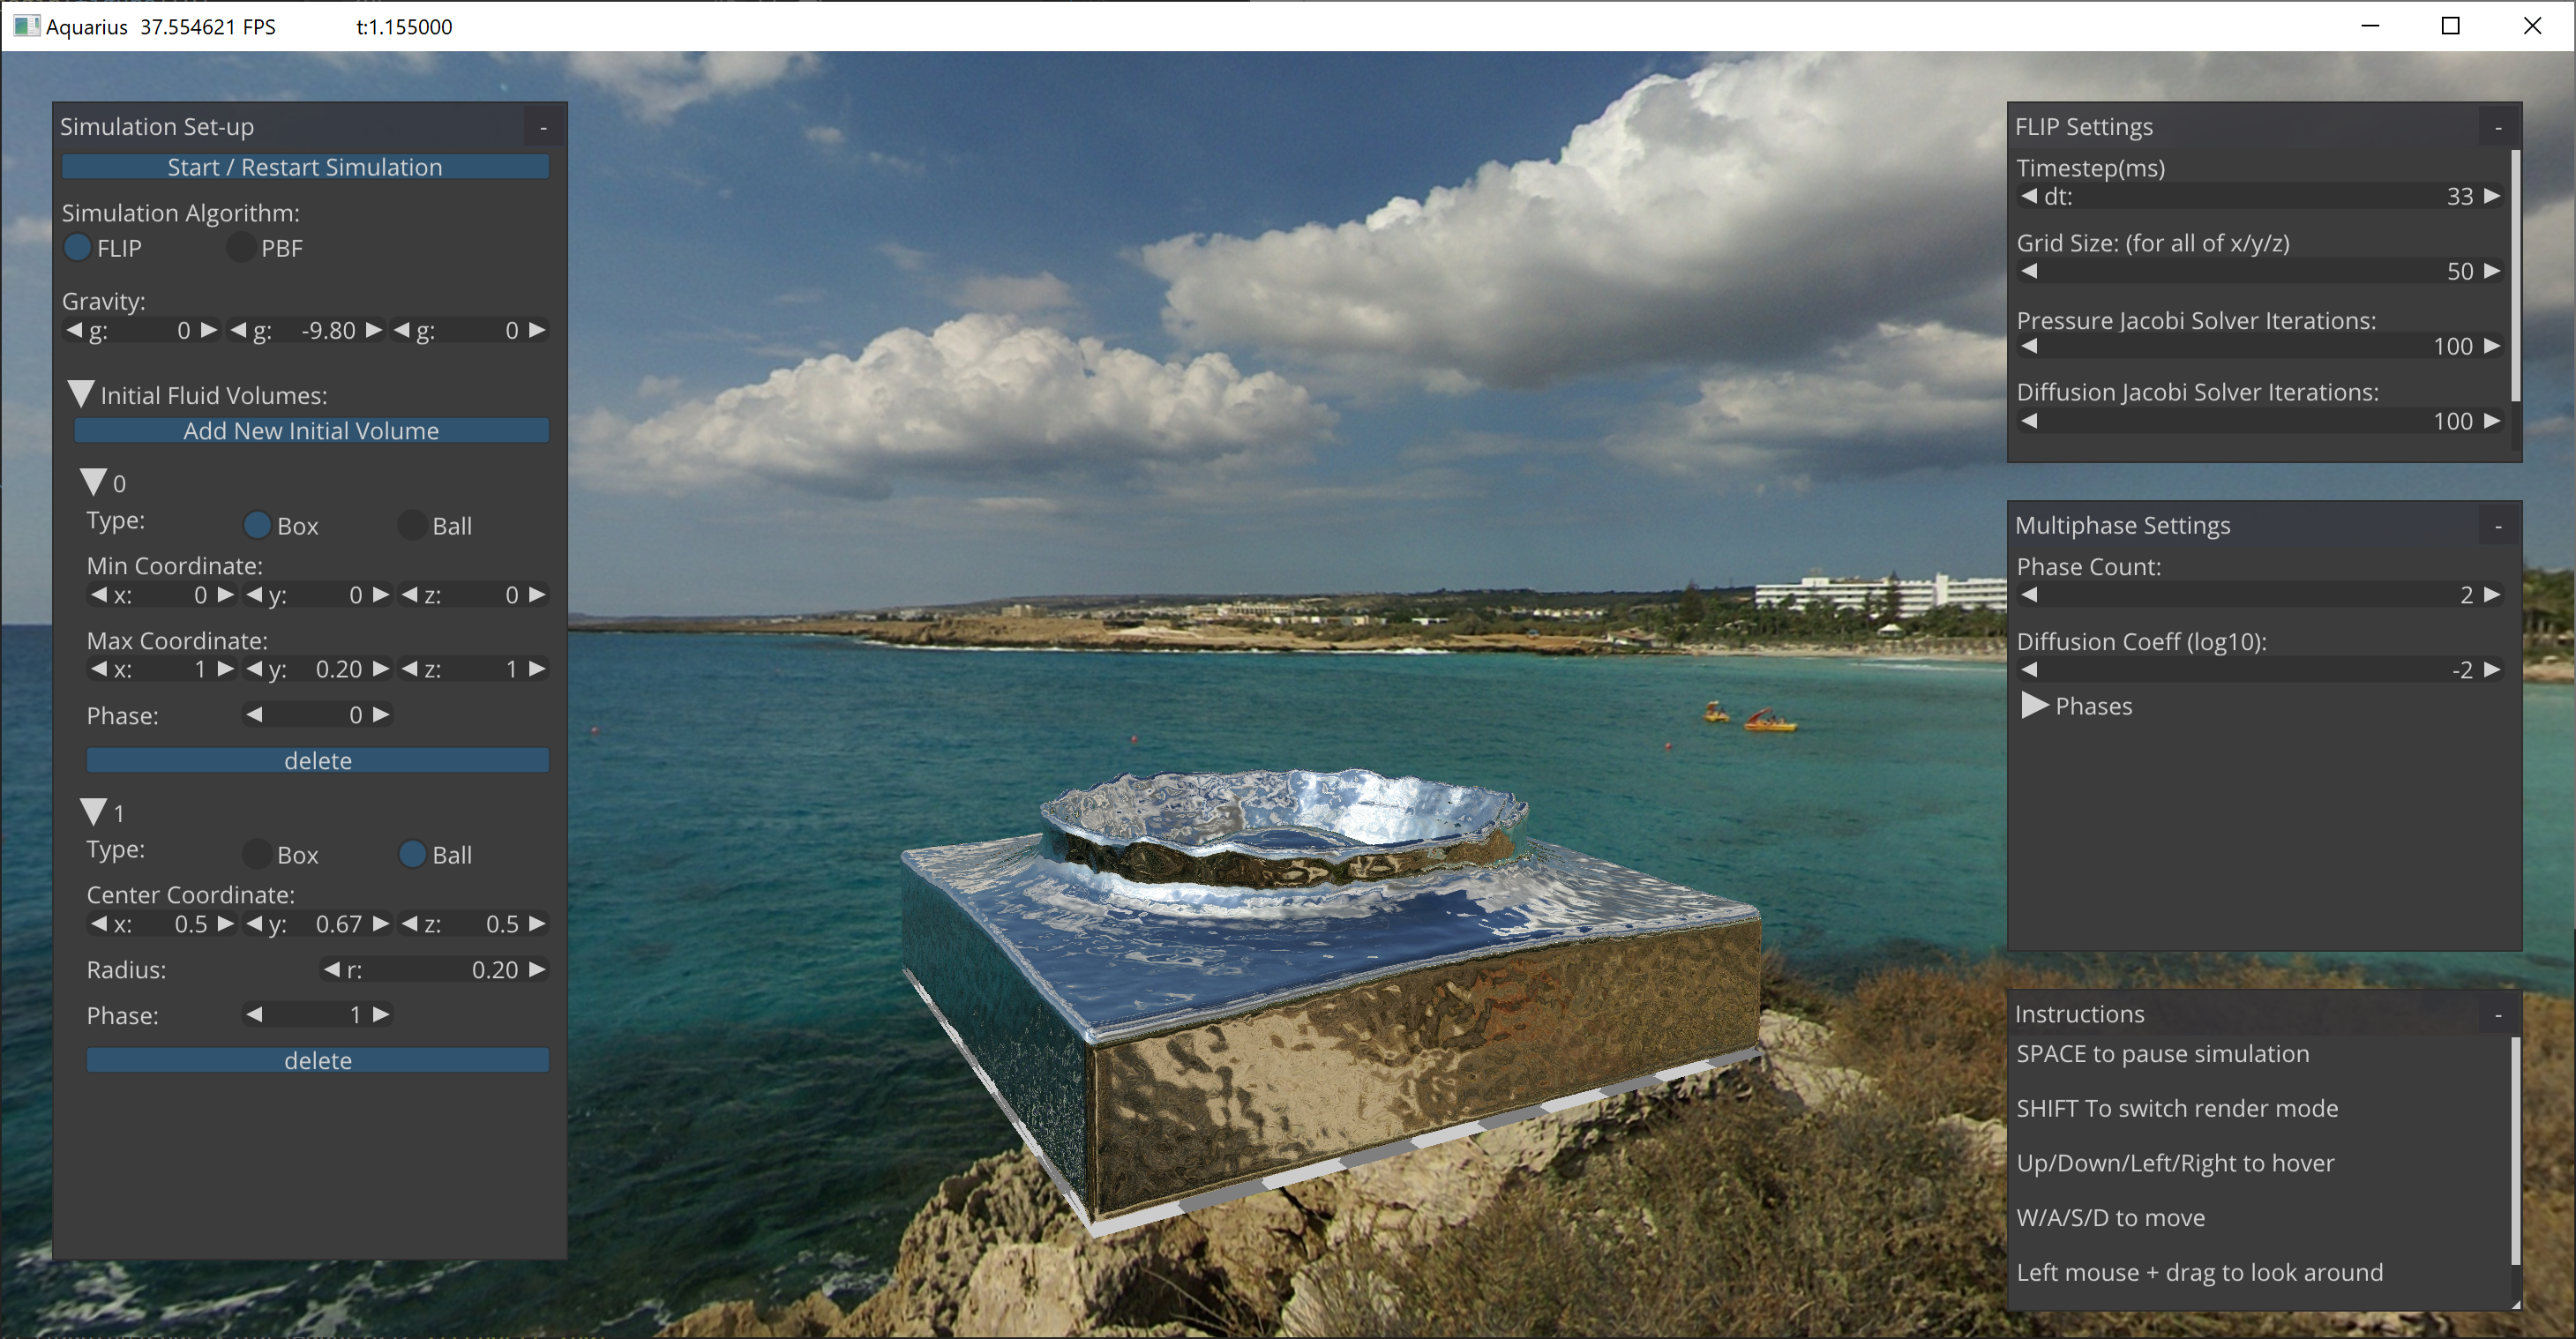
\includegraphics[width=10cm]{volume_cropped/reflection.png}
            \subcaption{The reflection}
    \end{minipage}
    
    \hspace{2pt}

    \begin{minipage}[t]{.65\linewidth}
            \vspace{0pt}
            \centering
            \includegraphics[width=10cm]{volume_cropped/blue.png}
            \subcaption{The thickness texture of the blue liquid. \\Brighter color indicates greater thickness.}
    \end{minipage}

    \hspace{2pt}
    
    \begin{minipage}[t]{.65\linewidth}
            \vspace{0pt}
            \centering
            \includegraphics[width=10cm]{volume_cropped/red.png}
            \subcaption{The thickness texture of the red liquid}
    \end{minipage}

    \hspace{2pt}
            
    
    \begin{minipage}[t]{.65\linewidth}
            \vspace{0pt}
            \centering
            \includegraphics[width=10cm]{volume_cropped/refraction.png}
            \subcaption{The refraction color.}
    \end{minipage}

    \hspace{2pt}

    \begin{minipage}[t]{.65\linewidth}
            \vspace{0pt}
            \centering
            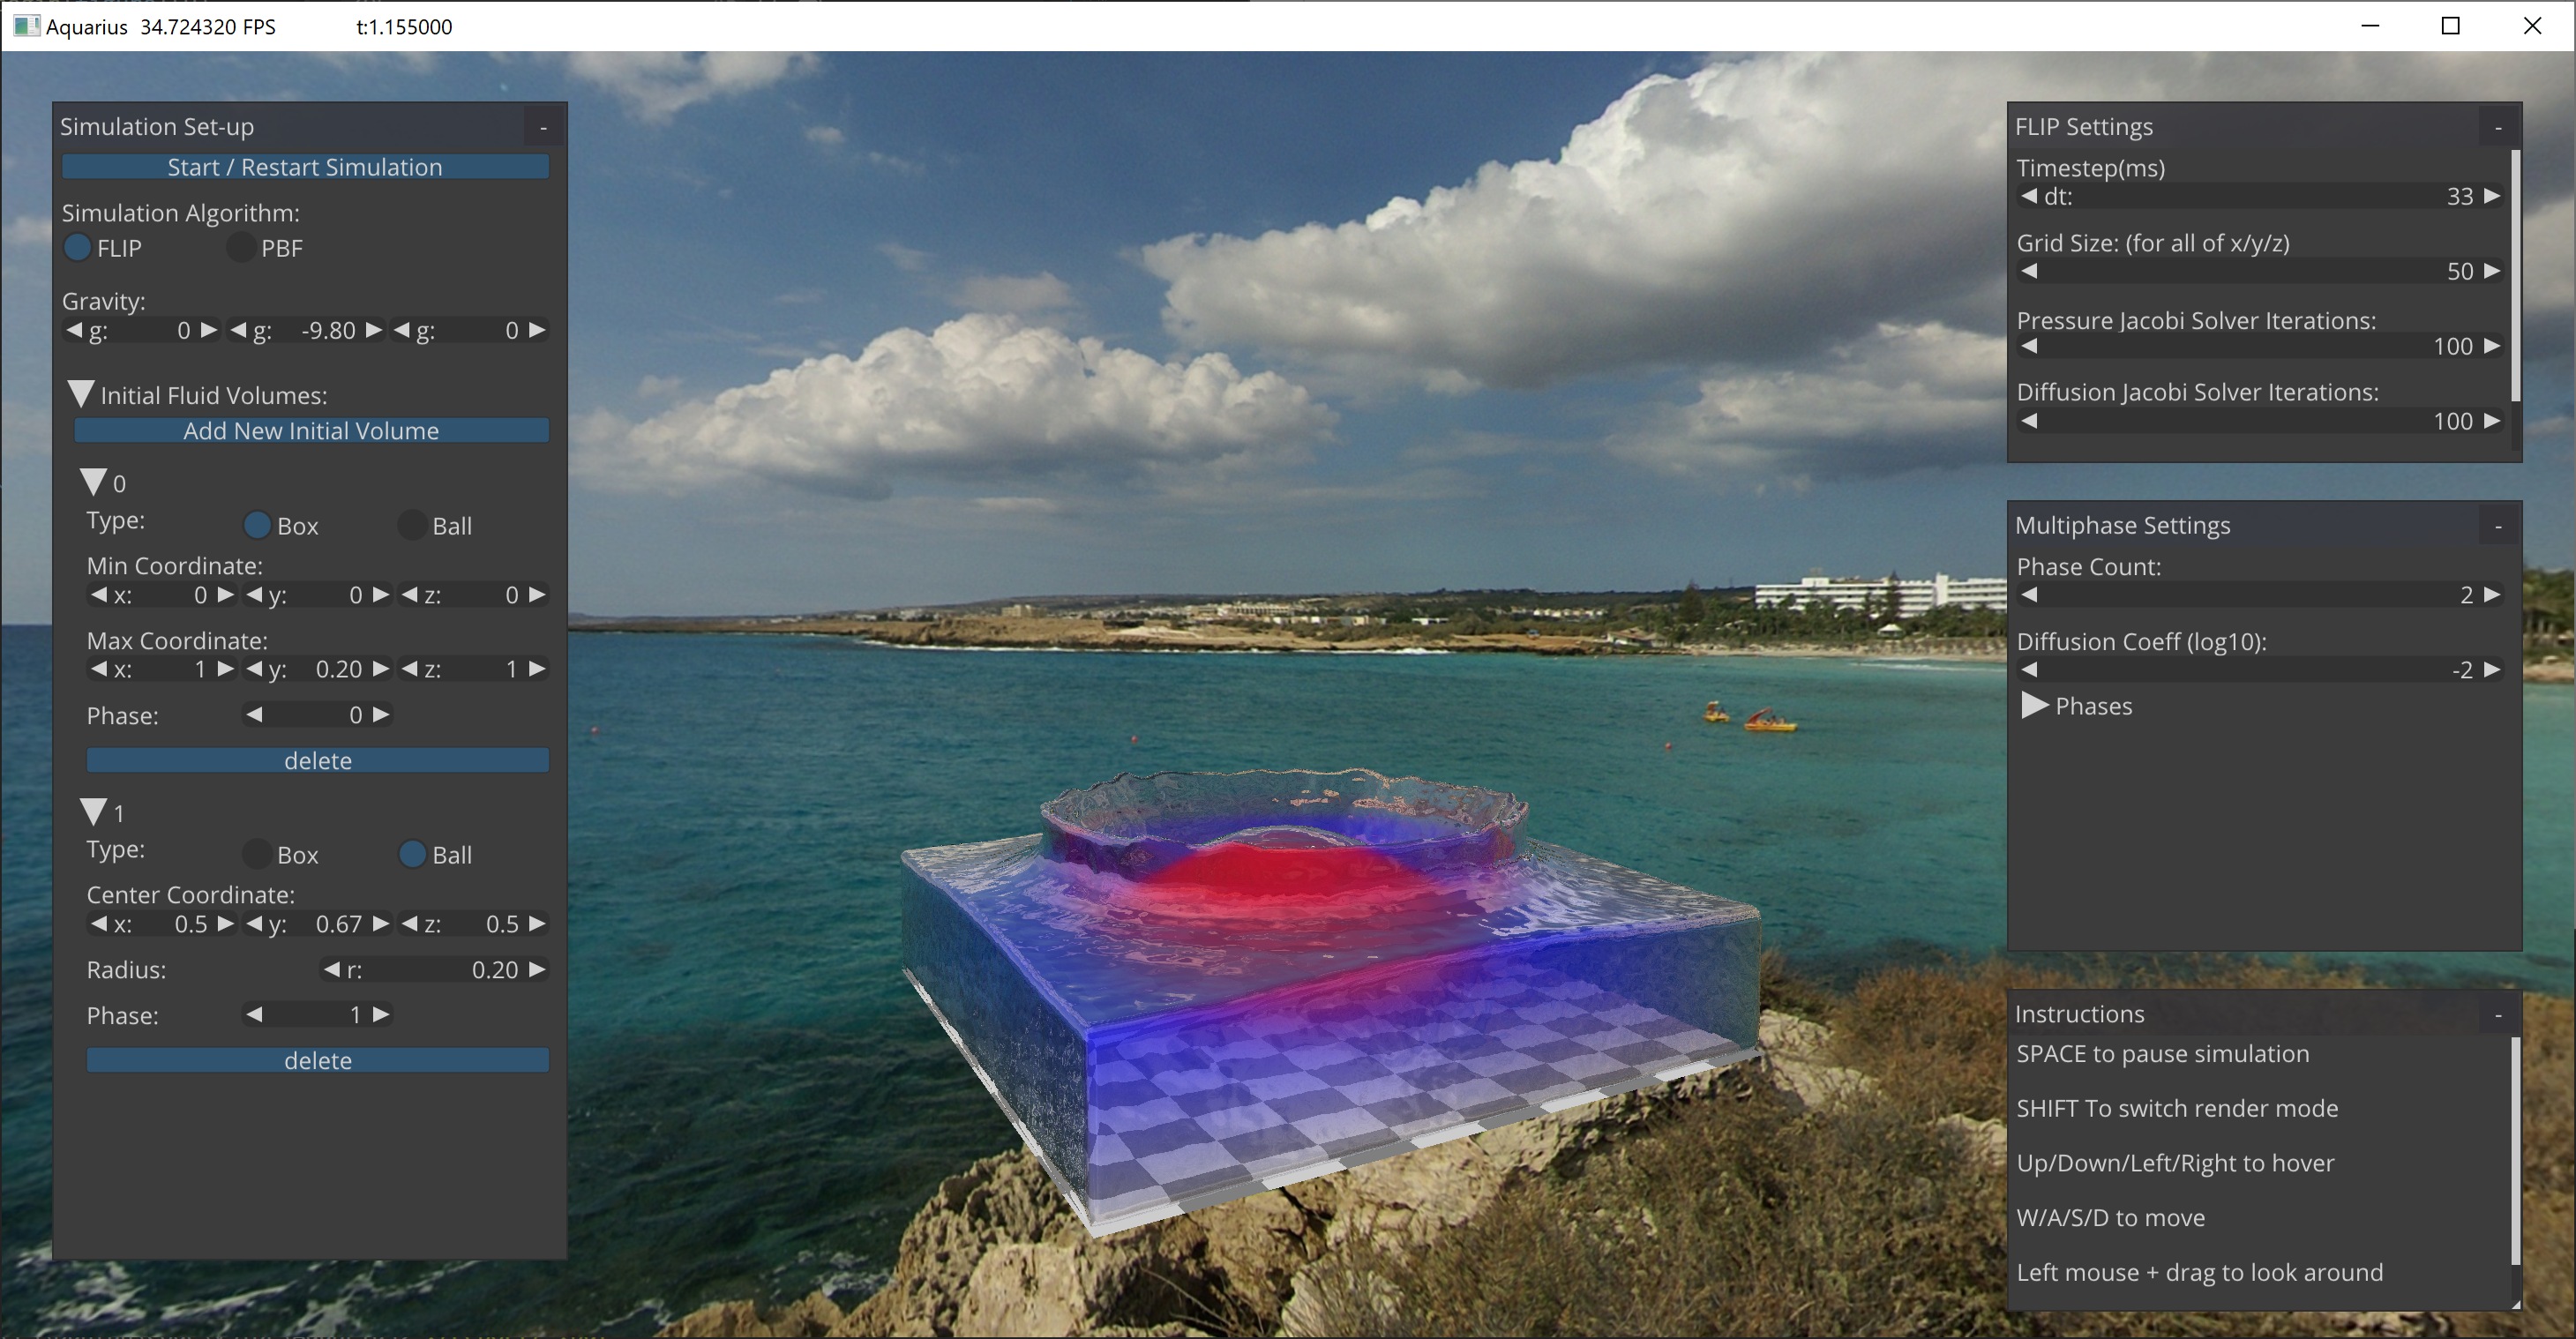
\includegraphics[width=10cm]{volume_cropped/final.png}
            \subcaption{Final result}
    \end{minipage}

    \hspace{2pt}
            

    \caption{Intermediary and final outputs of the renderer. The images show the moment after a large ball of red liquid falls into a box of blue liquid}
    \label{figure volume render}
\end{figure}


%\end{changemargin}
\addtolength{\topmargin}{.875in}


\chapter{Results}

Combining the FLIP implementation described in chapter \ref{chapter flip impl} and the render algorithms in chapter \ref{chapter render}, the software of this project is able to generate realistic images of many interesting simulations in real time. Some selected sequences of screenshots follow below.



\begin{figure}[H]
    \centering
    
    \begin{minipage}[t]{.24\linewidth}
        \centering
        \vspace{0pt}
        \includegraphics[width=3.5cm]{dambreak_cropped/0.png}
    \end{minipage}
    \begin{minipage}[t]{.24\linewidth}
        \centering
        \vspace{0pt}
        \includegraphics[width=3.5cm]{dambreak_cropped/1.png}
    \end{minipage}
    \begin{minipage}[t]{.24\linewidth}
        \centering
        \vspace{0pt}
        \includegraphics[width=3.5cm]{dambreak_cropped/2.png}
    \end{minipage}
    \begin{minipage}[t]{.24\linewidth}
        \centering
        \vspace{0pt}
        \includegraphics[width=3.5cm]{dambreak_cropped/3.png}
    \end{minipage}

    \caption{``Dam break" simulation}
    \label{fig dambreak}
\end{figure}

\begin{figure}[H]
    \centering
    
    \begin{minipage}[t]{.24\linewidth}
        \centering
        \vspace{0pt}
        \includegraphics[width=3.5cm]{diffusion_cropped/small0.png}
    \end{minipage}
    \begin{minipage}[t]{.24\linewidth}
        \centering
        \vspace{0pt}
        \includegraphics[width=3.5cm]{diffusion_cropped/small1.png}
    \end{minipage}
    \begin{minipage}[t]{.24\linewidth}
        \centering
        \vspace{0pt}
        \includegraphics[width=3.5cm]{diffusion_cropped/small2.png}
    \end{minipage}
    \begin{minipage}[t]{.24\linewidth}
        \centering
        \vspace{0pt}
        \includegraphics[width=3.5cm]{diffusion_cropped/small3.png}
    \end{minipage}

    \caption{Diffusion with coefficient $10^{-3}$}
    \label{fig diffusion 1e-3}
\end{figure}



\begin{figure}[H]
    \centering
    
    \begin{minipage}[t]{.24\linewidth}
        \centering
        \vspace{0pt}
        \includegraphics[width=3.5cm]{diffusion_cropped/big0.png}
    \end{minipage}
    \begin{minipage}[t]{.24\linewidth}
        \centering
        \vspace{0pt}
        \includegraphics[width=3.5cm]{diffusion_cropped/big1.png}
    \end{minipage}
    \begin{minipage}[t]{.24\linewidth}
        \centering
        \vspace{0pt}
        \includegraphics[width=3.5cm]{diffusion_cropped/big2.png}
    \end{minipage}
    \begin{minipage}[t]{.24\linewidth}
        \centering
        \vspace{0pt}
        \includegraphics[width=3.5cm]{diffusion_cropped/big3.png}
    \end{minipage}

    \caption{Diffusion with coefficient $10^{-2}$}
    \label{fig diffusion 1e-2}
\end{figure}

\section{Performance}

Performances of the software implemented in this project highly depend on the simulation parameters used. The most influential parameter is the grid resolution, which is required to be at least approximately $50^3$ to give pleasing visual results. The simulation and rendering algorithms take time linear to the number of cells occupied by fluids, which is cubic to the grid resolution in each dimension. In the following figure, the empirical framerate of the software is plotted against the resolution:

\begin{figure}[H]
    \centering

    \begin{tikzpicture}
        \begin{axis}[
            xlabel={Grid resolution},
            ylabel={FPS(frames per second)},
            xmin=30, xmax=60,
            ymin=0, ymax=80,
            xtick={30,35,40,45,50,55,60},
            ytick={10,20,30,40,50,60,70,80},
            xticklabels={$30^3$,$35^3$,$40^3$,$45^3$,$50^3$,$55^3$,$60^3$},
            ymajorgrids=true,
            grid style=dashed,
            width=12cm,height=7.3cm,
            legend style={at={(0.5,-0.1)},anchor=north}
        ]
        
        \addplot[
            color=red,
            mark=square,
            ]
            coordinates {
            (30,69)(35,68)(40,68)(45,67)(50,61)(55,44)(60,38)
            };
            \addlegendentry{Simulation only}
        
        \addplot[
            color=brown,
            mark=triangle,
            ]
            coordinates {
            (30,39)(35,38)(40,33)(45,27)(50,25)(55,21)(60,19)
            };
            \addlegendentry{Simulation + Singlephase Render}
        
        \addplot[
            color=blue,
            mark=diamond,
            ]
            coordinates {
            (30,30)(35,29)(40,26)(45,22)(50,20)(55,17)(60,15)
            };
            \addlegendentry{Simulation + Multiphase Render}
            
        \end{axis}
        \end{tikzpicture}
    
    \caption{Plot of framerate against grid resolution. Each simulation uses the identical initial condition, where 25\% of the domain is occupied with fluid. 100 Jacobi iterations are used in each time step. The tests are performed on a Microsoft Surface Book 2, with a i7-8650U CPU and a GTX 1060 GPU.}
    \label{fig FPS vs grid res}
\end{figure}


As a somewhat surprising observation, the computation time required to render a frame is actually considerably longer than the time taken to advance the simulation by one step. This is because, in order to generate a fine mesh, the resolution of the discrete grid of signed distance field is around 3 times the resolution of the MAC grid, which caused the surface reconstruction step (section \ref{section surface reconstruction}) to be rather expensive. Furthermore, multiphase rendering is noticeably more expensive than single-phase rendering, which is because if there is only one fluid phase, the particle-based optical thickness calculation (section \ref{subsection multiphase render}) is not required, and an approximation can be made using the tint colour of the fluid.

\section{Comparison with Existing Software}

The performance of the software created in this project is compared with a public CPU implementation of FLIP, namely the FLIP Fluids add-on\footnote{\url{https://blendermarket.com/products/flipfluids}} to Blender\footnote{\url{https://www.blender.org/}}. The same simulation parameters are used, and the programs are run on the same machine. Figure \ref{figure ball drop single}, \ref{figure ball drop multi}, and \ref{figure ball drop blender} show an example comparison. In these figures, a $50^3$ grid is used, which contains around $200k$ FLIP particles. While the CPU implementation in Blender takes around 1.1 seconds for each frame, the software of this project can perform simulation and rendering at $20$ FPS, which is substantially faster.

\gapM
\gapM
\gapM

\begin{figure}[H]
    \centering
    
    \begin{minipage}[t]{6.2cm}
        \centering
        \vspace{0pt}
        \includegraphics[width=5.7cm]{balldrop_cropped2/single0.png}
    \end{minipage}
    \begin{minipage}[t]{6.2cm}
        \centering
        \vspace{0pt}
        \includegraphics[width=5.7cm]{balldrop_cropped2/single1.png}
    \end{minipage}

    \vspace{0.5cm}

    \begin{minipage}[t]{6.2cm}
        \centering
        \vspace{0pt}
        \includegraphics[width=5.7cm]{balldrop_cropped2/single2.png}
    \end{minipage}
    \begin{minipage}[t]{6.2cm}
        \centering
        \vspace{0pt}
        \includegraphics[width=5.7cm]{balldrop_cropped2/single3.png}
    \end{minipage}

    \caption{Screenshots of a ``ball drop" simulation of the software created in this project.}
    \label{figure ball drop single}
\end{figure}

\newpage
\thispagestyle{empty}
\vspace*{-4cm}

\begin{figure}[H]
    \centering
    
    \begin{minipage}[t]{6.2cm}
        \centering
        \vspace{0pt}
        \includegraphics[width=5.7cm]{balldrop_cropped2/multi0.png}
    \end{minipage}
    \begin{minipage}[t]{6.2cm}
        \centering
        \vspace{0pt}
        \includegraphics[width=5.7cm]{balldrop_cropped2/multi1.png}
    \end{minipage}

    \vspace{0.5cm}

    \begin{minipage}[t]{6.2cm}
        \centering
        \vspace{0pt}
        \includegraphics[width=5.7cm]{balldrop_cropped2/multi2.png}
    \end{minipage}
    \begin{minipage}[t]{6.2cm}
        \centering
        \vspace{0pt}
        \includegraphics[width=5.7cm]{balldrop_cropped2/multi3.png}
    \end{minipage}

    \caption{Same simulation as figure \ref{figure ball drop single}, with 2 differently coloured phases.}
    \label{figure ball drop multi}
\end{figure}



\begin{figure}[H]
    \centering
    
    \begin{minipage}[t]{6.2cm}
        \centering
        \vspace{0pt}
        \includegraphics[width=5.7cm]{balldrop_cropped2/blender0.png}
    \end{minipage}
    \begin{minipage}[t]{6.2cm}
        \centering
        \vspace{0pt}
        \includegraphics[width=5.7cm]{balldrop_cropped2/blender1.png}
    \end{minipage}

    \vspace{0.5cm}

    \begin{minipage}[t]{6.2cm}
        \centering
        \vspace{0pt}
        \includegraphics[width=5.7cm]{balldrop_cropped2/blender2.png}
    \end{minipage}
    \begin{minipage}[t]{6.2cm}
        \centering
        \vspace{0pt}
        \includegraphics[width=5.7cm]{balldrop_cropped2/blender3.png}
    \end{minipage}

    \caption{Screenshots of Blender performing the same simulation as figure \ref{figure ball drop single}.}
    \label{figure ball drop blender}
\end{figure}


%\addtolength{\topmargin}{1.1in}

\chapter{Conclusions}
\label{chapter conclusions}

This project explored how modern GPUs can be programmed to efficiently simulate and render multiphase fluids. A software was built that was able to perform real time fluid simulation, and simultaneously render realistic images to be displayed. The project mostly focuses on parallelizing existing algorithms, but invents an original algorithm for performing fast multiphase fluid volume rendering. The software created is named \textit{Aquarius}, and its full source code is available at \url{https://github.com/AmesingFlank/Aquarius}.


\section{Limitations \& Future Work}
\label{section future work}

During the development of this project, many ideas emerged which would all bring more significance to this project. Unfortunately, the time permitted did not allow them to be explored. The following are a few valuable features that the software doesn't yet support, but could be added in future endeavors.



\begin{itemize}
    \item Viscosity.
    
    This project focused on fluids that follow the Euler equations, ignoring the effect of viscosity as described in the full Navier-Stokes equations. While not problematic for water-like liquids, many other interesting visual effects of fluids (e.g melting chocolate) are only possible with viscosity. 
    

    \item Solid-fluid coupling
    
    In the real world, the motion of fluids almost always induces or is induced by the motion of solids. Modelling the coupling between solid and fluid allows more useful simulations. 

    \item Caustics, shadows, and foams
    
    The renderer built in this project is far from complete, there are still a lot of optical features that are not captured. The curved shapes of liquids can cause the refracted light to be focused onto certain areas, creating an alternating pattern of brightness and darkness, known as caustics and shadows. Also, fast moving liquids sometimes have small regions that traps volumes of air, creating foams. These phenomenons are common in real life, and supporting them in the renderer can significantly increase the realism of the images generated.

    \item Performance Improvements
    
    The FLIP simulation code in this project is very efficient. However, other parts of the program, especially the renderer, still has a large room for improvements. With more work, the performance of the software could definitely be improved.


    \item Publishing as a library
    
    In its current form, the software created by this project has limited practical use. However, with some extra engineering, the code could be turned into a distributable library that can be used to perform fluid simulation in other projects. Specifically, it could be adapted into a plugin for popular game engines such as Unity or Unreal, so that game programmers can use it to easily incorporate real time fluids in their work. 
    
\end{itemize}

\section{Personal Reflections}
Working on this project has been a gratifying experience. The topic is very exciting, and there was so much to that I learnt during the process. Apart from the improvements mentioned in \ref{section future work}, which I wish I could have made more progress in, I am in general very happy with and proud of the results I achieved.

When I submitted the proposal of this project in February 2019, it was purely based on interest as I had no previous experience and understanding of fluid simulation. So, the first thing I had to do in this project was to learn about the physics of fluids. As a pure computer science student, this proved challenging at first, because the mathematics courses that CS students took virtually did not discuss any vector calculus. In the Easter vacation of 2019, I spent a substantial amount of time catching up with vector calculus and fluid dynamics, which was difficult, but layed the ground for my future efforts.

Before I started reading academic papers on the topic, I read a book called \textit{Fluid Simulation for Computer Graphics}\cite{bridson2015fluid}, written by Robert Bridson, one of the leading experts in the field. This book gave a really good advice: always start by writing a 2D simulator, before moving on to 3D. I did follow this advice, and took it one step further: I started by writing code that only runs on CPU, before moving on to a GPU implementation. This was definitely a good idea because, considering the level of complexity of my GPU implementation right now, it would have been impossible for me to implement it correctly when I was still very unfamiliar with the problem at hand. A lesson learnt here is that for complicated tasks, a good way to start is by building a simple prototype.

One of the biggest challenges that I faced in this project is the performance of my program. When I first ported my CPU 2D fluid simulator code to GPU, the simulation was only running at an embarrassing 7 frames per second, without even incorporating any sophisticated rendering. I was quite anxious about this, because I really wished to achieve real time simulation and rendering, and that is for 3D. At that time, the performance problem was caused by the pressure solver (\ref{section enforce incompressibility}), which was taking tremendously long to solve the pressure Poisson equation. After weeks of careful analysis, a few optimization tricks, and some helpful directions pointed out by my supervisor, Professor Joe Pitt-Francis, I eventually resolved this issue. There isn't a specific moral in overcoming this obstacle, but I certainly learnt a lot about numerical computation and GPU optimization because of it.

I absolutely enjoyed learning about fluids and coding a simulator, but, somewhat surprisingly, I also enjoyed writing this report very much. Not only was I able to talk about a project that I worked passionately on, but as I reiterated the methods I used, I cleared up a few technical details which I did not completely understand. Although, I found it quite stressful to obey the 10,000 word limit. There are a few mathematical details and some experimental methods (e.g PBF and PCISPH), which I spent a considerable amount of time working on, but sadly could not fit into this report.

This project is possibly the biggest intellectual endeavor I have made in my years at Oxford(though waiting to be surpassed by my 4th year project), and I find it to be an unmissable part of my education. Through this project, I was exposed to many spectacular areas of computer graphics that I did not know existed, and I was familiarized with the techniques essential to these studies. I have grown as a computer science student because of this project.

%now enable appendix numbering format and include any appendices
%\appendix
%\include{appendix1}
%\include{appendix2}


%next line adds the Bibliography to the contents page
\addcontentsline{toc}{chapter}{Bibliography}
%uncomment next line to change bibliography name to references
%\renewcommand{\bibname}{References}
\bibliography{refs}        %use a bibtex bibliography file refs.bib
\bibliographystyle{plain}  %use the plain bibliography style

\end{document}

